\documentclass{article}

\usepackage{fancyhdr}
\usepackage{ragged2e}
\usepackage{graphicx}
\usepackage{caption}
\usepackage{geometry}
\usepackage{amsmath}
\usepackage{rotating}

\usepackage{listings}
\usepackage{color}

\definecolor{dkgreen}{rgb}{0,0.6,0}
\definecolor{gray}{rgb}{0.5,0.5,0.5}
\definecolor{mauve}{rgb}{0.58,0,0.82}

\lstset{frame=tb,
  language=Java,
  aboveskip=3mm,
  belowskip=3mm,
  showstringspaces=false,
  columns=flexible,
  basicstyle={\small\ttfamily},
  numbers=none,
  numberstyle=\tiny\color{gray},
  keywordstyle=\color{blue},
  commentstyle=\color{dkgreen},
  stringstyle=\color{mauve},
  breaklines=true,
  breakatwhitespace=true,
  tabsize=4
}

\setcounter{secnumdepth}{1}

\usepackage{chngcntr}
\counterwithin{figure}{section}

\renewcommand*{\thepage}{C\arabic{page}}

\pagestyle{fancy}
\lhead{ACME Robotics}
\chead{\#8367}
\rhead{\ifcontents Contents \else Week \thesection \fi}

\newif\ifcontents
\contentstrue

\makeatletter
\renewcommand{\@seccntformat}[1]{}
\makeatother

\begin{document}\tableofcontents\newpage\contentsfalse\clearpage \newpage \section{Week \thesection} 
\subsection{Business Goals}
\paragraph{B1: Write fundraising letters}
 Write two fundraising letters, one for existing sponsors and one for new sponsors. 
\paragraph{B2: Discuss the Engineering Notebook process with both teams}
 Have an in-depth discussion about the Engineering Notebook process with both ACME and ARES. 
\newpage
\subsection{B1: Write fundraising letters}

Since establishing ARES Robotics, the two teams plan to fundraise and go to outreach events together. Since ACME has more experience with writing fundraising letters, Emma was tasked with writing them. She wrote one letter for existing sponsors and then modified it to explain the teams and FIRST for potential sponsors. There are four levels of sponsorship for ACME and ARES. All of them give sponsors benefits, such as their company name/logo on the team website, company name/logo on the side of the robot, and having a private presentation to the sponsoring company. ACME had these support levels last year as well and they worked very well because the sponsor could choose their support level based on what incentives they wanted. The ARES captain, Sean, looked over the letter and approved it. After, the teams developed a potential sponsor list. and wrote another fundraising letter targeted to new sponsors.  

\subsection{B2: Discuss the Engineering Notebook process with both teams}

With all of the new team members on ACME (and with ARES being a rookie team) it made sense to discuss the Engineering Notebook as a group. Emma made a presentation on the general setup and format of an Engineering Notebook (EN) and presented it to both teams. Then they split up into teams and Kelly discussed the specifics of the ACME EN with members. He went over how ACME uses Overleaf to format the EN and how this year members will be writing their entries straight into Overleaf. \\

The Captains decided to write all of the EN entries in Overleaf because it is more simplistic process than what they did the previous year (i.e. writing entries in Google Sheets and then transferring them into \LaTeX). Since ACME is a smaller team this year, it was fairly simple to teach everyone how to use the platform. Having the entries written directly into Overleaf also allows the EN to be ready for competition earlier because each week can be generated when members finish writing their entries. 
\clearpage \newpage \section{Week \thesection} 
\subsection{Business Goals}
\paragraph{B1: Develop a schedule for the first part of the season}
 Decide on a schedule that tailors to the needs of the team for the first tournament.
\paragraph{B2: Setup a task tracking system}
 Decide on a task tracking platform.
\subsection{Hardware Goals}
\paragraph{H1: Develop intake prototypes}
The game this year requires the robot to be able to sort the gold and silver minerals. We need to come up with and test various ideas for ways to pick up and sort out the two types of minerals.
\paragraph{H2: Investigate possible drivetrain designs}
 Research different drivetrains and decide which would be suitable for this game.
\paragraph{H3: Develop Drivetrain Prototypes}
 Work on a drivetrain prototype at the Build Weekend.
\subsection{Software Goals}
\paragraph{S1: Test vision software}
 Develop vision software to detect the gold particle
\paragraph{S2: Experiment with new motor controller features}
 Play with new motor controller features to see what benefits they have.
\newpage
\subsection{B1: Develop a schedule for the first part of the season}

After the Build Weekend, the team got together to discuss the schedule for the first part of the season. The schedule was based around the robot goals that members want to accomplish for the first qualifier. There were several other factors to consider as well, such as leaving time to fabricate, assemble, practice auto and driving. With these thoughts in mind, here is the schedule the team developed. 

\subsection{B2: Setup a task tracking system}

Last year, the team used a whiteboard in the robotics room to keep track of tasks that needed to be completed. This worked great, except, unless you took a picture of it after every meeting, you could not easily access it remotely. Which is why this year, ACME captains decided to use Jira to keep track of tasks. Jira is an online task tracking product developed by Atlassian. Team captains have the capability to assign tasks to members, as do mentors. The team has found that this software works very well for them and will continue to use it in the future. You can see the Jira dashboard in Figure \ref{fig:jiradash}.

\begin{figure}
    \centering
    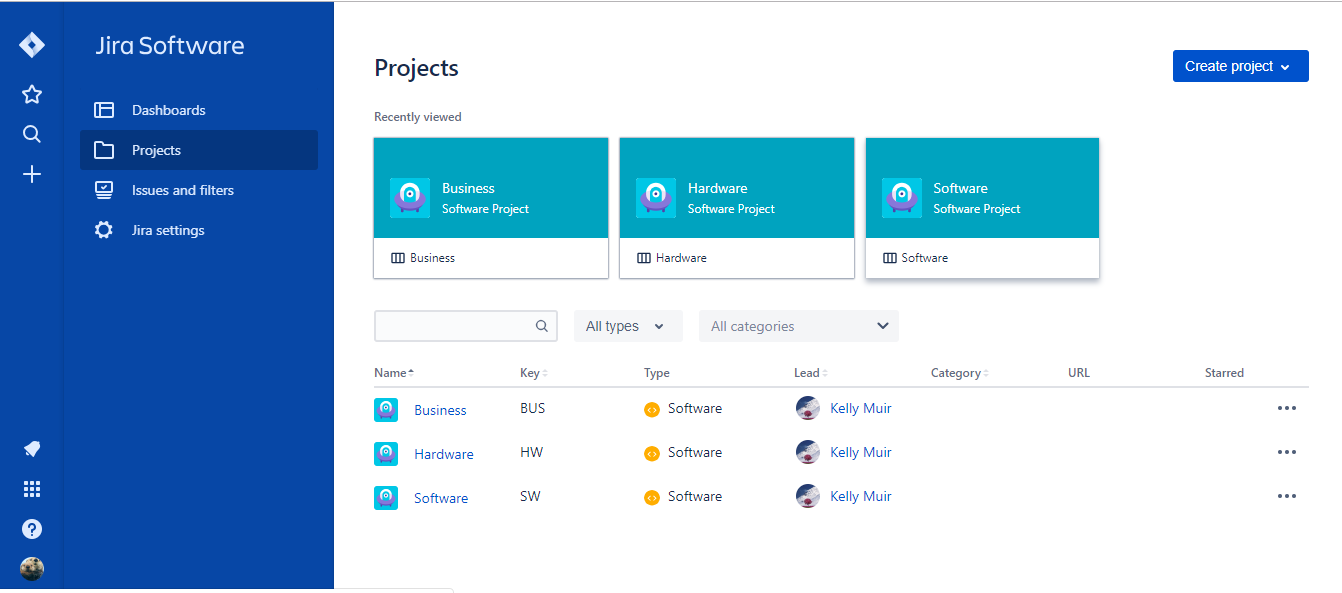
\includegraphics[width=.6\textwidth]{02_09-10/images/jiradash.png}
    \caption{Jira Dashboard}
    \label{fig:jiradash}
\end{figure}
\subsection{H1: Develop intake prototypes}

After the whole team watched the game video, several members began prototyping mechanisms to intake and sort cubes. Because the game requires the robot to pick up minerals that are inside the crater, the robot either needs to be able to climb over the crater to intake the minerals, or extend some sort of intake over the crater wall. 

Kelly decided to try developing an intake mechanism that would allow the robot to stay outside of the crater, and reach over the wall, which would allow the team to continue using a mecanum drivetrain, for its increased maneuverability. The first concept they thought of was to extend a rake in front of the robot, on linear slides, that would pull the minerals back to the robot and up the crater wall. The rake would have tines spaced a little bit under 2.75 in apart, so the silver minerals would be pulled back, but not the gold minerals. This would allow the robot to cycle back and fourth between the crater and the silver depot, to score minerals as fast as possible. When this prototype was tested, Kelly found that the gold minerals could still be pulled back, when a silver mineral would get stuck in the tines of the rake, so the rake concept would not work to sort out the minerals. 

The next concept Kelly tested was a spinning surgical-tubing intake, similar to ACME's Velocity Vortex robot. By spinning the two stages of the intake in opposite directions, the minerals would first be pulled into the robot, and then pushed against the rake, expelling the gold minerals and allowing the silver to pass into the robot. This design relied on the fact that if the intake was extended over the outer boarder of the crater, any minerals in it would be inside the crater, and thus not subject to the two mineral maximum. This worked well to pull in the minerals once they were brought to the top of the crater wall by the rake, but the transition between the two counter-rotating brushes caused the minerals to get stuck, or rejected prematurely. 

After watching videos of robots from Res-Q, the last FTC game to involve the same game elements, Kelly decided the surgical tubing intake was worth pursuing, because it could quickly bring minerals to the top of the robot one at a time, which would be necessary for sorting them out. Kelly built a new prototype that had the surgical tubing whips mounted directly over one another and rotating the same direction. Ashlin built a acrylic back plate and funnel that would guide the minerals up the intake, and allow only one to pass through the top at once. Kelly built a simple sorting system that consisted of two parallel bars mounted far enough apart to allow the gold to pass through, but not the silver. When this was combined with the spinning intake, the minerals would be sucked up into the robot, and then divided into gold and silver. 

After Jon finished the prototype for the intake he began to find the optimum distances the needed to be from the ground, crater edge, and edge of the robot. This is because these measurements are vital for CADing and fabrication. Jon found that the optimum distance from the robot to the roller was 7 inches. While the optimum distance from the floor to the roller was 4 inches. 
\begin{figure}
    \centering
    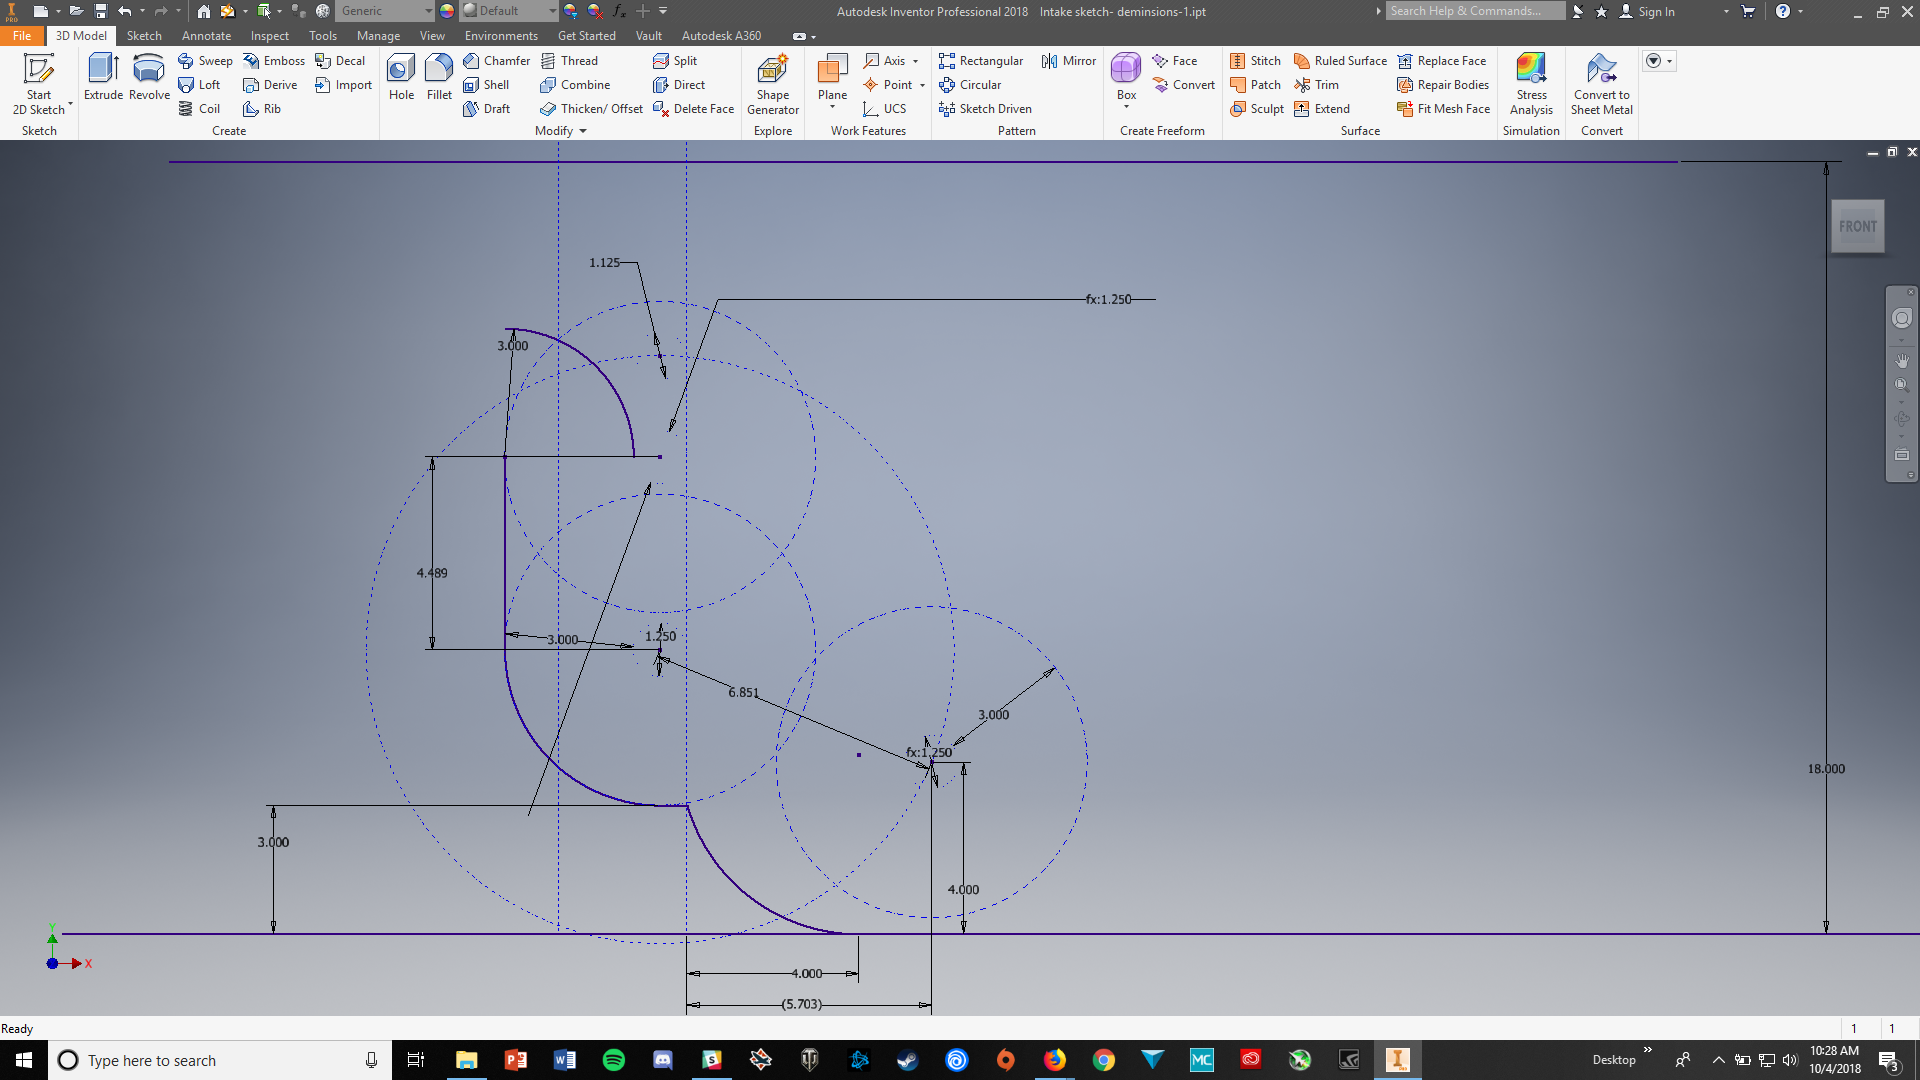
\includegraphics[width=.6\textwidth]{02_09-10/images/intakesketch.png}
    \caption{Deploy-able intake dimensions}
    \label{fig:intake}
\end{figure}



\subsection{H2: Investigate possible drivetrain designs}

Given that a good drivetrain is vital for a successful robot, the team needed a solid design. The team decided there were two ways of going about creating a good drivetrain for the Rover Ruckus challenge. The first was to design a drivetrain capable of going inside the crater. The team thought this might be a good idea seeing as the intake design would be simpler and we could traverse all areas of play. This would need to be a drivetrain with very good traction, torque, and durability. For this purpose the team looked into a drop-center tank design (WCD) or a tracked design. Suspension was also considered. These were considered because both WCD and tracked designs are very effective at traversing rough or bumpy terrain. Like the crater rim. Jon did research in this area and found a simple suspension (bell crank) design and sketched a few ideas for a tracked drive train (fig 0.1). After discussing these together, and WCD, the team decided that going into the crater was probably not necessary. Thus, the team stopped development on these ideas and continued pursing the second way of going about designing a drive train.



\begin{figure}
    \centering
    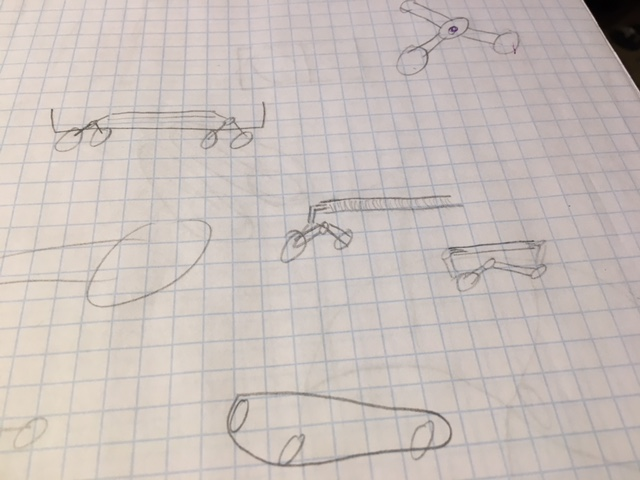
\includegraphics[width=.6\textwidth]{02_09-10/images/IMG_0256.JPG}
    \caption{Bell crank suspension and tracked drivetrain sketches}
    \label{fig:drivetrain sketches}
\end{figure}



\subsection{H3: Develop Drivetrain Prototypes}

Shawn and Ben worked on developing a rocker bogie drivetrain to test. The drivetrain used two different rotation points on both sides to be able to get over things, such as the crater wall. They used a picture from the Internet to assist in the construction of the drivetrain. After it was finished, the drivetrain worked as expected but wasn't quite within the size constraints. Sadly, the drivetrain had to be taken apart. 

\subsection{S1: Test vision software}

Finding the gold particle at the beginning of the autonomous posed many challenges for the software team. Modifying a python vision script from the Relic Recovery season, Emma and Kelly were able to successfully detect the gold particle. However, the problems started when they realized that with the robot starting above the ground, the camera would have full view of the crater full of gold particles behind the line of particles they were trying to detect, as seen in
Figure \ref{fig:camera}.

After discussing possible solutions, including identifying the three particles first (both silver and gold), Emma decided to experiment with camera angles from approximately five inches above the field. Without having the field nor the mounting point on the robot, Emma tried her best to find the optimal position for the camera, although a final position will need to be determined once the robot is complete. 

Although there are different ways to solve this problem using programming, for simplicity's sake, Emma is hoping to troubleshoot more with the camera when the field arrives sometime in the next week. As they already have functional code, it would be beneficial to only have to position the camera correctly. 

\begin{figure}
    \centering
    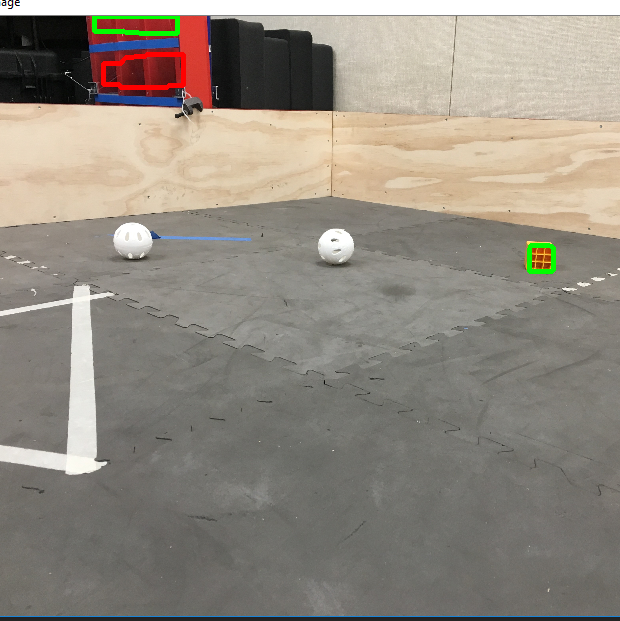
\includegraphics[width=.6\textwidth]{02_09-10/images/originalcameraposition.png}
    \caption{Original Position of the Camera}
    \label{fig:camera}
\end{figure}



\subsection{S2: Experiment with new motor controller features}

New motor functionality added with v4.0 of the SDK and the new Rev Expansion Hub firmware has the ability to have a PIDF control loop on the Rev Hub itself. This means that rather than commanding some vague `power' to the motor, and then having to empirically determine the relationship between this power and the velocity of the motor, you can directly command a velocity, and the control loop on board the hub will match that velocity regardless of voltage droop. After upgrading the firmware in the hubs and testing this functionality with a lone motor, Kelly re-wrote the MecanumDrive class to take advantage of it. After deploying this to the Relic Recovery robot, Kelly found that the robot was much easier to control. Without any feed-back control on the robot controller side, the robot was very stable, and it was much easier to move the robot slowly, because the hub would now do the work of closing a loop around the velocity of the robot.\clearpage \newpage \section{Week \thesection} 
\subsection{Hardware Goals}
\paragraph{H1: Work with intake prototypes.}
 Test intake prototypes. 
\paragraph{H2: Develop a Team Marker}
 Design a team marker that will be used at the tournaments.
\newpage
\subsection{H1: Work with intake prototypes.}

After looking further into the dual flywheel intake design, Jon and Kelly decided this was not a practical option because it would be difficult to fit onto the robot and create an efficient chain setup. Kelly and Jon then decided to go with a swing down roller design, as this would be easy to fit into the existing design and will likely work just as well. After deciding this, Jon built a prototype for this new intake. 

\begin{figure}
    \centering
    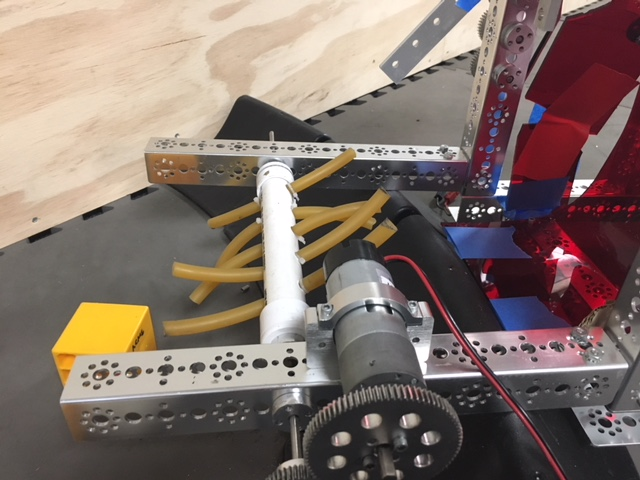
\includegraphics[width=.6\textwidth]{03_09-17/images/IMG_0262.JPG}
    \caption{Deploy-able intake prototype}
    \label{fig:my_label}
\end{figure}

\subsection{H2: Develop a Team Marker}

Shawn and Ben were tasked with developing a team marker. The team marker should fit within the size constraints and, ideally represent something about the team. Ben and Shawn decided to make a prototype anvil marker that could roll. Ben sketched out an anvil in his notebook and measured the height of cardboard. Based on this measurement, he divided the drawing into equal sections that were that height. Shawn the cut out the cardboard pieces and they pieced it together.\clearpage \newpage \section{Week \thesection} 
\subsection{Hardware Goals}
\paragraph{H1: Sorting Mechanism}
 Design a sorting mechanism to sort the minerals. 
\paragraph{H2: Investigate potential lift designs}
 Figure out which lift designs would work the best for the robot. 
\paragraph{H3: Design lift gearbox}
 Design a lift gearbox that can move the lift quickly and can lift up the robot. 
\subsection{Software Goals}
\paragraph{S1: Integrate the hub feedforward functionality into trajectory followers}
Integrate the new feedforward functionality into the trajectory code for auto paths.
\newpage
\subsection{H1: Sorting Mechanism}

Ashlin, Aidan and Kelly worked on the process for sorting the cubes from the balls. The first idea was a mechanical sorting system that would function like a coin sorter, allowing the cubes to fall through while the balls rolled past. This design was discarded because it took too much space and was not consistent. A new sorting system involved a color sensor and a U shaped cup. In figure \ref{fig:Sorter Version 2} the new system is shown connected to a prototype robot. The cube or ball would roll into the U-cup and then be read by the color sensor. The U-cup would then rotate about 135 degrees clockwise or counterclockwise to deposit the cube or ball in the corresponding cartridge. This idea did not work because there were not available servos that could rotate the required 270 and the system required too much space. This failed sorting system led to a third sorting system that was based around version two but took up less space and did not have to rotate as much. The final design, figure \ref{fig:Final Sorting Mechnism}, allowed the ball or cube to go into the rotating circle part where it would be read by the color sensor and then a servo would rotate the circle part about 45 degrees clockwise or counterclockwise to deposit it in the corresponding cartridge. This system worked significantly better because it allowed there to be only 90 degrees of rotation needed by the servo, the process would be significantly shorter, and the whole system could be condensed to take up no more than a 6 inches.

\begin{figure}
    \centering
    \includegraphics[width=.6\textwidth]{04_09-24/images/sorter.jpg}
    \caption{Sorter Version 2}
    \label{fig:Sorter Version 2}
\end{figure}

\begin{figure}
    \centering
    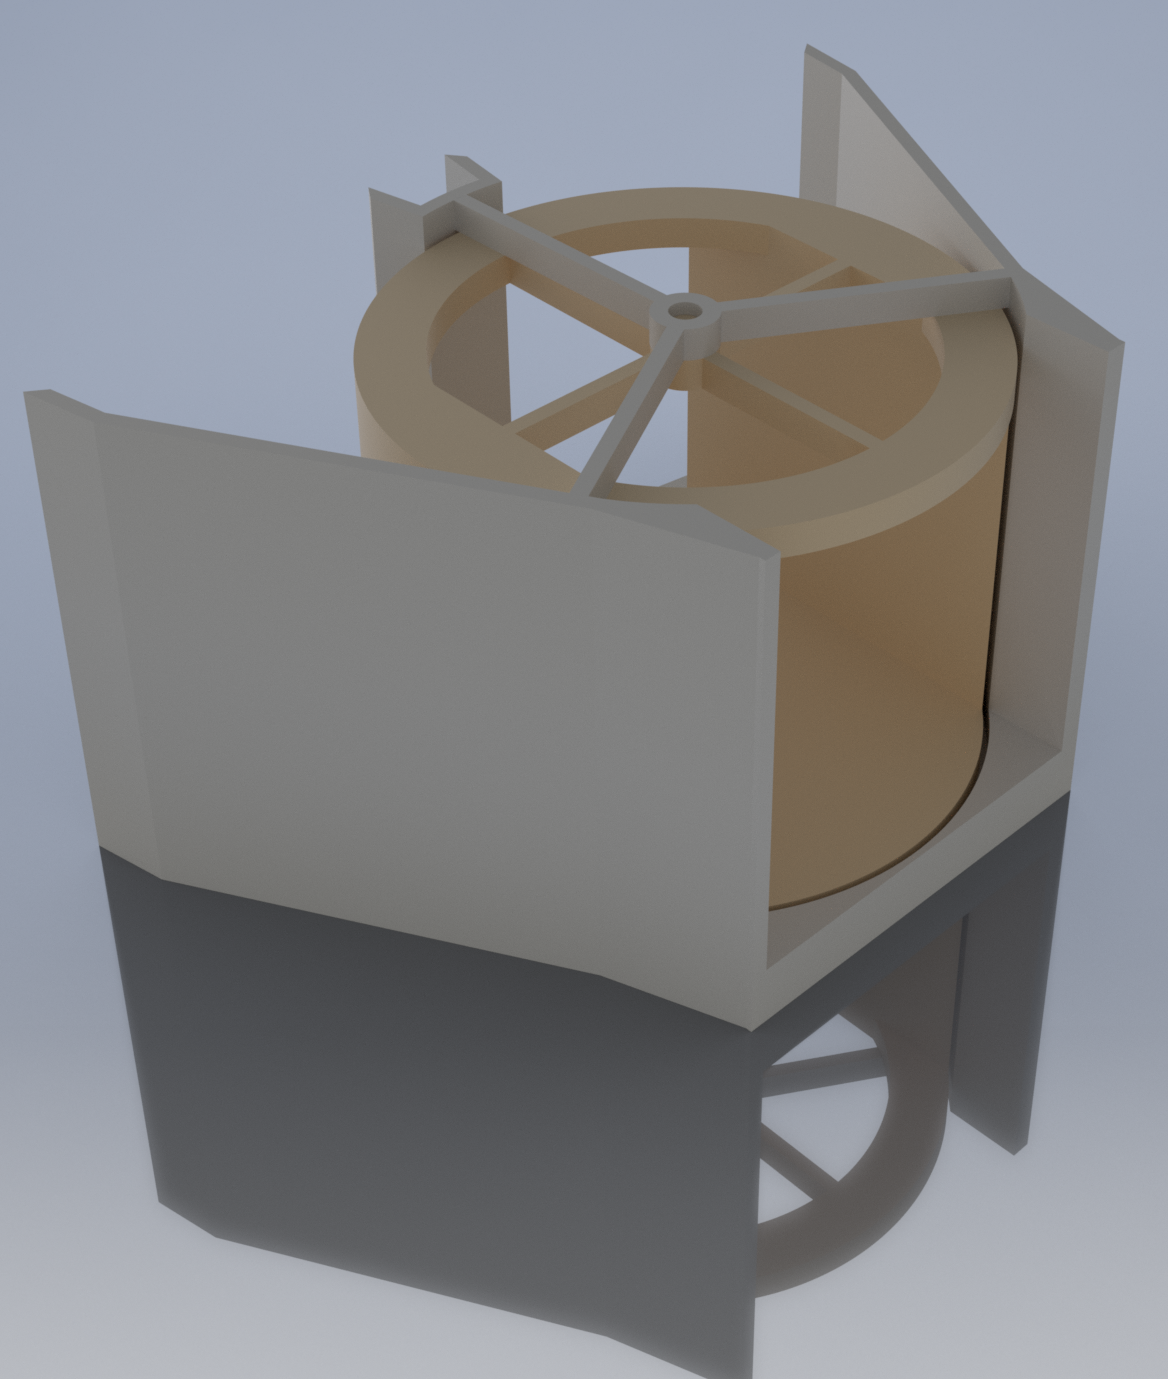
\includegraphics[width=.6\textwidth]{04_09-24/images/sorter2.png}
    \caption{Final Sorting Mechanism}
    \label{fig:Final Sorting Mechnism}
\end{figure}

\subsection{H2: Investigate potential lift designs}

The lift is going to be one of the most important mechanisms on the robot this year, as it is required for both scoring and latching. It will also need to be capable of moving very quickly, when carrying minerals to the top of the lander, and powerful enough to lift the entire robot off the ground at the end of the match. Because the team had only used Rev linear motion kits and drawer slides before, Kelly investigated the other options available for linear motion. Any potential solution needed to be capable of extending to the top of the lander, which is 32 inches off of the surface of the field, which would require two 16 inch stages, or three shorter stages. Because the lander bracket is only about four inches above the top of the robot, the mechanism that will attach to the lander only needs to be mounted to the first stage, meaning that any subsequent stages do not need to be as robust, as they will only ever bear the weight of the scoring system, not the robot itself. These requirements are quite similar to the FRC challenge last year, Power Up, which required teams to lift blocks above their robot to score, and then hang from a bar. Team 254, in particular, had a design that is super promising. It consisted of two fixed rails, a box-like first stage than ran between the fixed rails, and a smaller second stage carriage that ran within the first stage frame. Since this overall form factor fit all of the requirements, the team decided to settle on it for now, and investigate hardware that it could be constructed from. Team 254 constructed their lift out of square aluminum tubing and bearings that would roll against the surface, making it super fast and smooth. While this provides the best performance, the main drawback to this approach is the difficulty in manufacturing the brackets that mount the bearings to the tubing to the tolerances necessary to make everything run smoothly. If any parts are out of alignment or not parallel, then it gets a lot harder to move the lift. Another pre-fabricated option that many teams used last year to extend their relic arms over the field wall is Actobototics x-rail. The x-rail has a v-shaped groove on each side of its cross-section, allowing a v-bearing to run in the track. This would cut down on the number of bearings needed for the lift, because each pair of bearings can constrain the lift in two dimensions, not just one. If the bearings are aligned so that the majority of the forces go radially into the bearings, rather than axially, than it could be quite robust. Kelly configured the lift using these parts, and then put together a list of parts necessary to construct the lift. Because the brackets are pre-fabricated, the tolerances are much tighter than could be achieved if the team manufactured them. 

\subsection{H3: Design lift gearbox}

Another goal for the lift was finding a suitable gearbox that would fit all of the requirements for the lift. During this process, Kelly decided against a shifting gearbox because of the neccecary complexity, which meant that at least two motors would need to be used to get sufficient torque to lift the robot at the gearing neccecary to make the lift fast enough. A ratchet would also need to be involved so that the robot could hang from the lander without powering the motors, making it easier to start and end the match. After researching options for a dual-motor gearbox, Kelly settled on a Versa Planetary from VexPro, because it could use a dual motor input to drive one gearbox from two motors, removing the need to join the two motors after the reduction and was modular meaning any custom gear ratio could be created; it could also be integrated with a ratchet kit to allow for one-way rotation when lifting off the ground. After assuming that the robot would weigh the full 20 kg, and requiring the motor to be able to accelerate it at 2g, a 25:1 reduction would be neccecary. This should be enough to lift the scoring mechanism to the top of the robot in 1.5s, so the gearbox should be sufficient. Kelly added the necessary parts to the order sheet.
\subsection{S1: Integrate the hub feedforward functionality into trajectory followers}

Before, with each update of the control system, the trajectory would return a target velocity at that given moment, which would be multiplied by the empirically determined coefficient that would convert it to a power to command to the motor. The target position of the trajectory would be compared to the actual position of the robot, and a PID loop would use this error to correct the power commanded to account for the error. Now, the velocity returned by the trajectory is directly commanded to the motor, and the rev hub does the work of converting that to a voltage that is applied to the motor. The positional error still is accounted for, but now by correcting the commanded velocity, not the commanded power. Even with very low gains on the Positional PID loop, this yielded markedly better results than the previous trajectory follower, because of the new functionality in the Rev Hubs. The second necessary change to the trajectory follower was the way error was calculated. Previously, positional error was split into two components, axial and lateral, but the axial error was always parallel to the robot's heading, and the lateral error was always perpendicular to it. Because the new pathing system treated the drive completely holonomically, this no longer made sense, because when the robot was strafing, the axial error would be normal to its direction of travel, but when the robot was driving forward, the axial error would be tangent to its direction of travel. If the robot was moving through a curve with constant heading, always on the path but 1 inch behind where it wanted to be, the error would first be primarily axial, and then primarily lateral, which would cause strange behaviours when these errors are fed into separate PID loops. To counteract this, Kelly changed it so that the axial error was always tangent to the robot's direction of travel, and the lateral error was always normal to the robot's direction of travel. This improved the usefulness of the error measurements.
\clearpage \newpage \section{Week \thesection} 
\subsection{Business Goals}
\paragraph{B1: Discuss Gracious Professionalism}
 Discuss the important FIRST value of Gracious Professionalism with both teams.
\subsection{Hardware Goals}
\paragraph{H1: Continue Developing The Team Marker}
 Creating a releasing mechanism for the team marker. 
\paragraph{H2: Drivetrain decision}
 Decide on the design for the drivetrain.
\paragraph{H3: Develop custom lift}
 Further investigate possible lift designs and weigh the pros and cons of each. 
\subsection{Software Goals}
\paragraph{S1: Start Working on Lift Kinematics}
 Begin to work on lift kinematics for the robot.
\newpage
\subsection{B1: Discuss Gracious Professionalism}

Although ACME members from last year were well versed in the ways of Gracious Professionalism, the new members - and ARES members - were not. As Gracious Professionalism is the underlining value of FIRST, Emma and Kelly decided to give a presentation on the subject. Pulling up a Google Slides presentation in the Drive, Emma was able to write a fairly comprehensive guide on how to be a Gracious Professional. After having Kelly read it over, and spending some time developing the Flowers Dialectic, Kelly presented it to both teams. The teams had a great discussion about how and how not to behave at competition, as well as how to be a Gracious Professional in their everyday life. The only thing this presentation could not totally explain was how rewarding it can be to practice these values. The team especially saw this last year at the Northern California Regionals, when they helped their friends, team 5214: Tech Support, by buying them an emergency servo. The team ended up being on the winning alliance because of it.  
\subsection{H1: Continue Developing The Team Marker}

Shawn and Ben hadn't quite finished the anvil when they realized that the marker had no deployment mechanism and it looked super bad. They then decided to go with just a cube with a loop that could be dropped by a servo over the side. Shawn was tasked with making the block and he made it out of acrylic. Then Ben used basic Tetrix to make a servo mechanism that would unhook the cube and make it fall. Ben built the mechanism and found that a lot of servos didn't work.

\begin{figure}
    \centering
    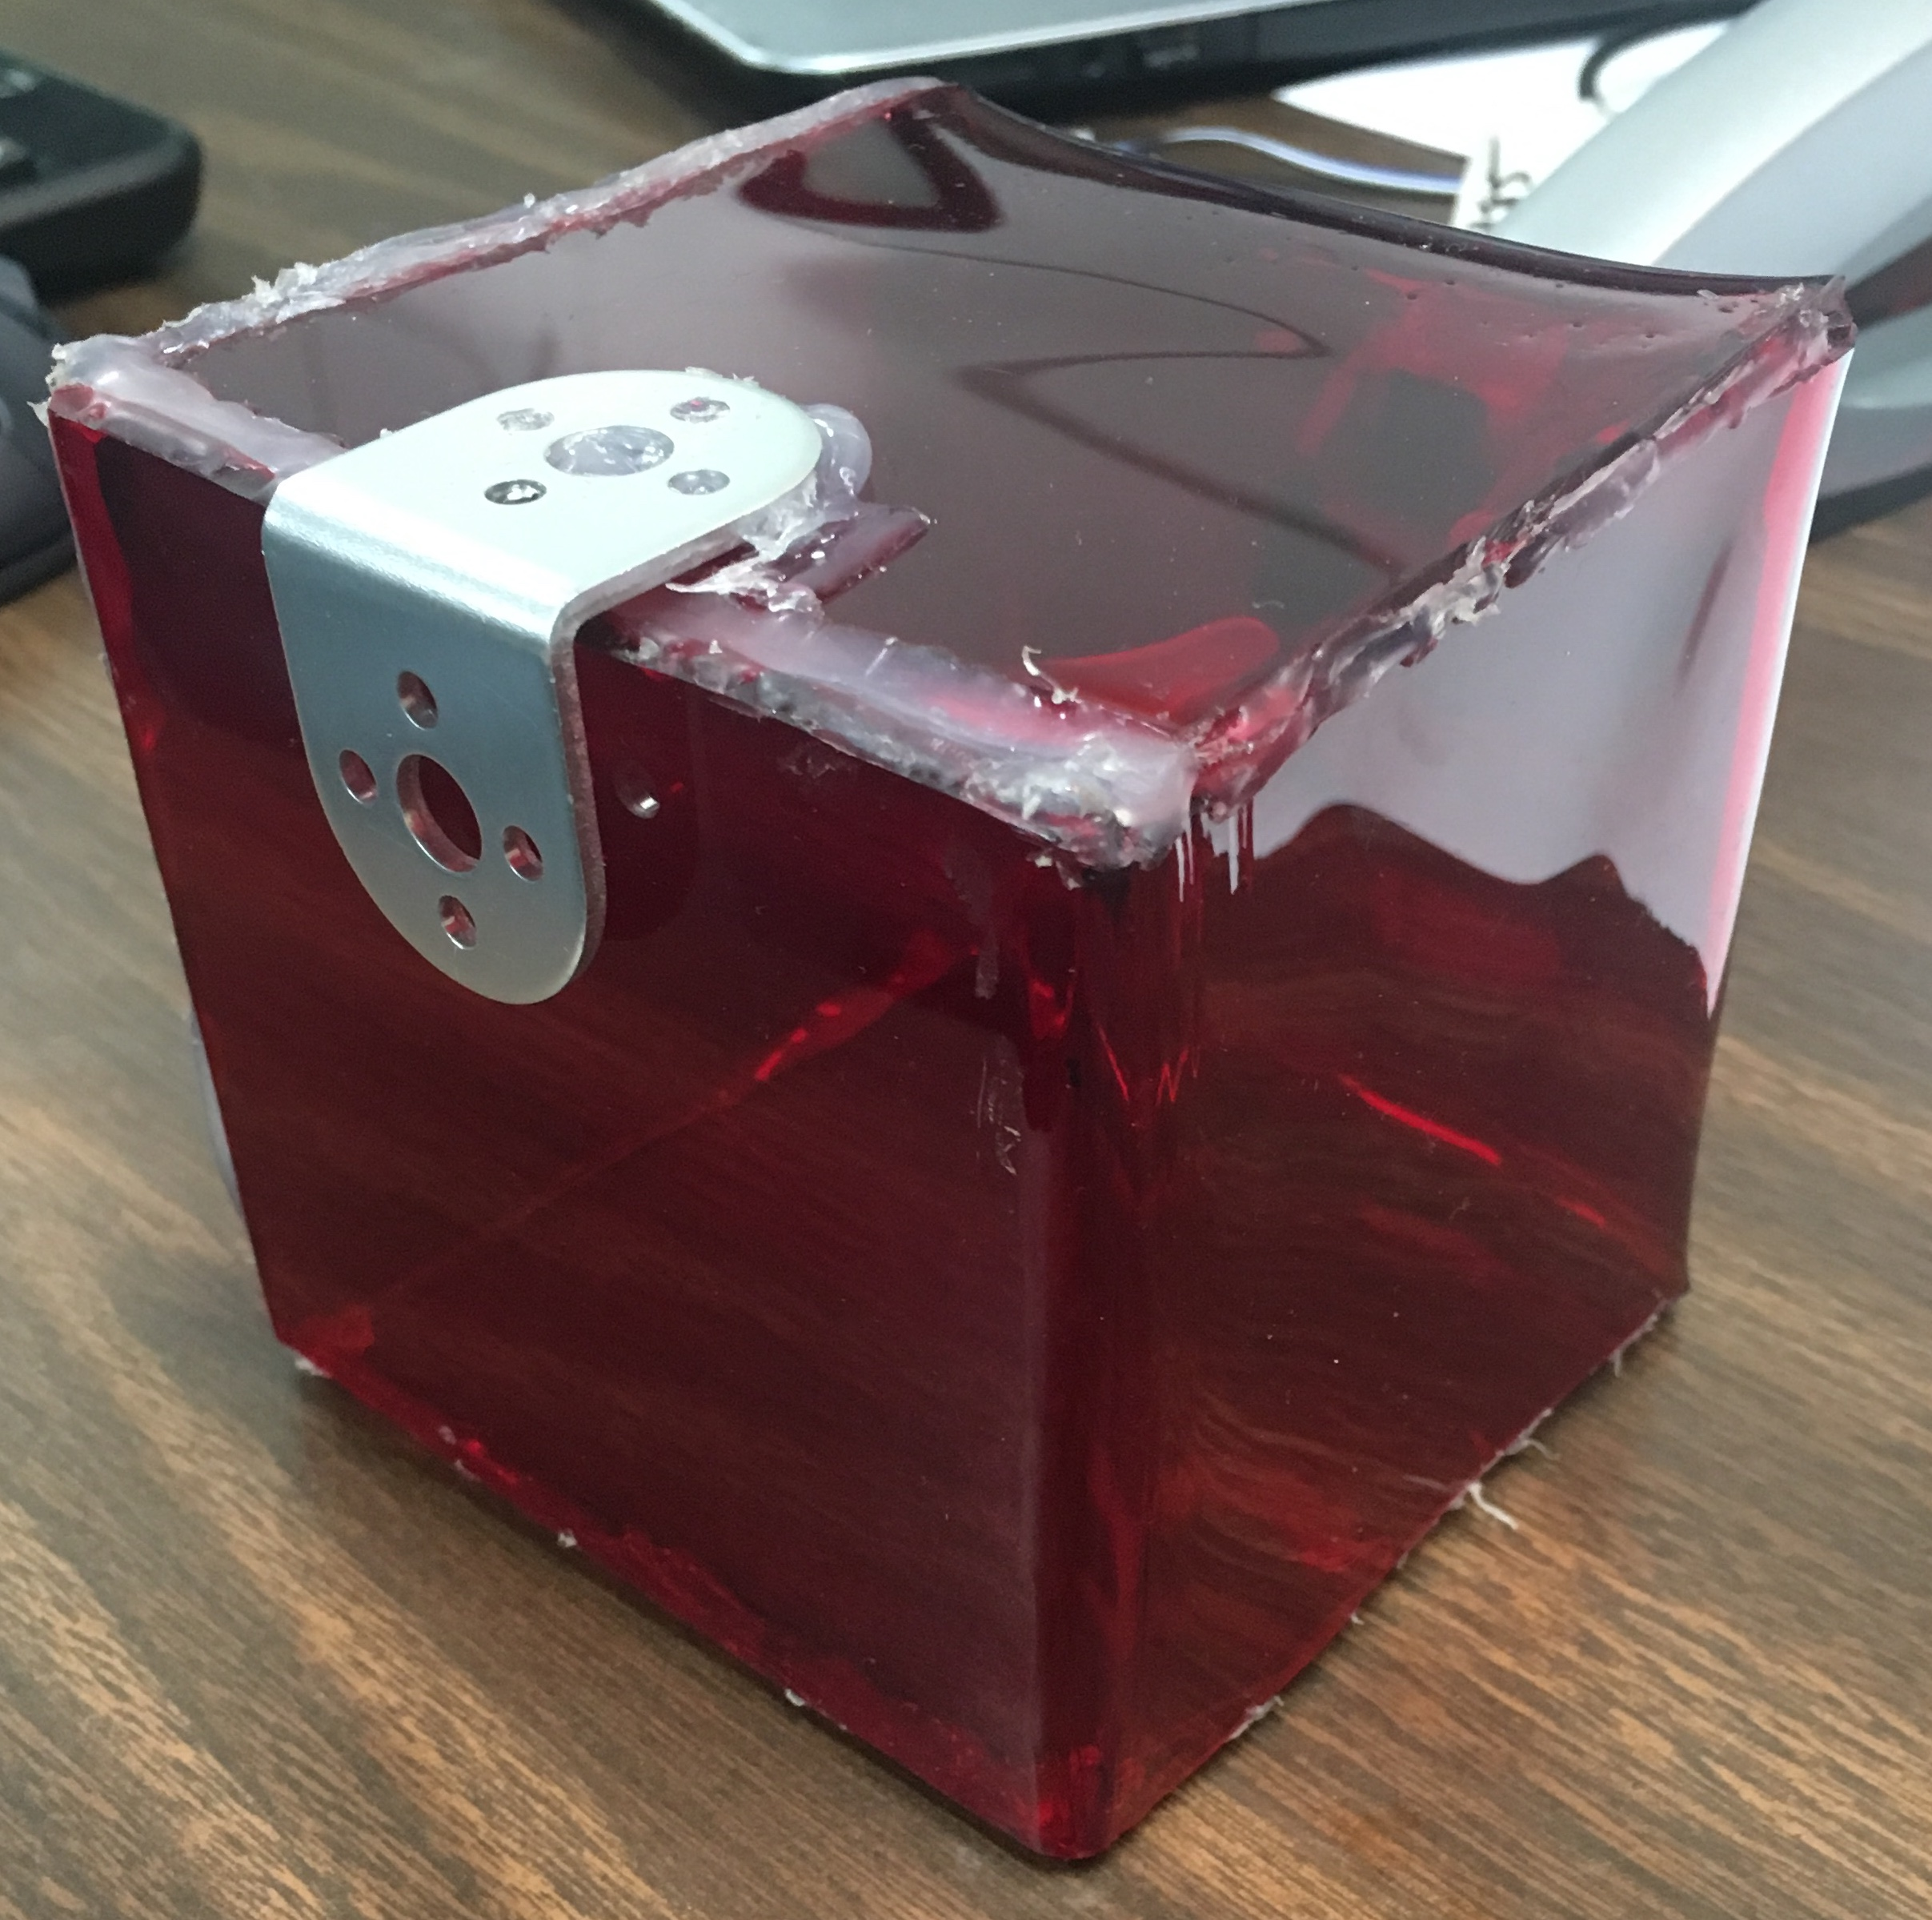
\includegraphics[width=.6\textwidth]{05_10-01/images/cube.jpg}
    \caption{Acrylic Cube}
    \label{fig:cube}
\end{figure}



\subsection{H2: Drivetrain decision}

The entire team made a matrix to help weight the pro and cons of the prototype drive-trains and already proven styles. The matrix took a lot in to consideration, such as agility, size, strength, traction, and maneuverability. The results of the matrix was a mecanum style drive-train driven by orbital 20 gearbox and belts. We choose this style because of its high speed, agility, and maneuverability, the downside to this style drive-train is the traction, which in turn can make playing defense a lot hard, compared to a none mecanum drive-train.  

\subsection{H3: Develop custom lift}

The x-rail lift design would work, but Kelly still wanted to investigate the 254-style lift, with square tubing, bearings, and custom bearing blocks. While more labor-intensive and harder to pull off, the end result would be better than with x-rail if it turned out correctly. Where the x-rail only needed bearings on one side, because the v-bearings would be able to resolve both radial and lateral loads, normal bearings can only resolve radial loads, so bearings will have to be placed on at least three sides to constrain the lift in both dimensions. Since the lift is composed of two mirrored parts, connected by the frame of the first stage, Kelly could get away with only running bearings along three sides of each tube, excluding the outer one, because the bearings in the y-axis would push the two sides against each other, preventing the lift from shifting side-to-side. Each bearing assembly would consist of four bearings, two on either side of the tube pinching it, and two next to each other running along the inside of the tube. Kelly began the CAD by making 1 in by $\frac{1}{2}$ in by $\frac{1}{16}$ in wall aluminum tubing in 16 inch lengths. One of these would be mounted to the drivetrain, and the other would make up the vertical portion of the first stage, rolling along the fixed one. A bearing assembly would go at the top of the fixed one and the bottom of the moving one, keeping the bearings as far apart from each other as possible, distributing the load and stabilizing the lift. The inner carriage would be made out of a H-shaped arrangement of more tubes, with a bearing assembly mounted at the top and bottom of each side of the H. After considering mounting the bearings by sandwiching the tube between two machined plates, Kelly realized this would not support the inner bearings, so decided on machined blocks that would be fixed to the tube with rivets. The blocks would have a quarter inch hole on the side for attaching the pinching bearings, and hole at the top where a bolt would connect the two blocks and support the inner bearings. After assembling this, Kelly found there was not enough room on the vertical portion of the first stage for both sets of bearings to roll against it, so it was neccecary for them to be swapped out for one inch by one inch tubes instead. 
\subsection{S1: Start Working on Lift Kinematics}

This week, Emma began to work on lift code for the robot. There were several things that the team needed the lift to do. First there needed to be a driver controlled portion of the code so that drivers could manually lift and lower the lift. The other modes needed were run to position; where the lift could go to a certain position and hold position; so that the lift will stay at the position it is currently at. Emma used an enum for this. Enums are excellent for storing data that doesn't present as textual or numerical data, which is why they are ideal for this situation. Emma also learned how we use motion profiling on the robot. It is important to integrate motion profiling into the lift so that movements are as smooth and precise as possible. Here is the code that Emma wrote this week.
\begin{lstlisting}[language=Java]
    private enum LiftMode{
        DRIVER_CONTROLLED,
        HOLD_POSITION,
        RUN_TO_POSITION;

    }
            switch (liftMode){

    public void goToPosition(double position){
        liftProfile = MotionProfileGenerator.generateSimpleMotionProfile(
                new MotionState(0, 0, 0, 0),
                new MotionState(position, 0, 0, 0),
                1, 1, 1 //find real values eventually
        );
        liftMode = LiftMode.RUN_TO_POSITION;
        startTime = System.currentTimeMillis();

    }
\end{lstlisting}
A motion profile is generated every time goToPosition is called. Emma is hoping to work on the other modes next week.
\clearpage \newpage \section{Week \thesection} 
\subsection{Hardware Goals}
\paragraph{H1: Sorter CAD}
 CAD the sorter.
\paragraph{H2: Develop X-rail based lift}
 Develop a CAD model of the x-rail based lift.
\paragraph{H3: CAD Lander Clamp}
 Create a latch in CAD that will be used to attach to the lander. 
\paragraph{H4: Finalize robot design}
 Discuss the final robot design with the team.
\subsection{Software Goals}
\paragraph{S1: Continue working on lift kinematics}
 Continue developing software for the lift.
\newpage
\subsection{H1: Sorter CAD}

Ashlin and Aidan continued to finalize the sorting system for the robot and completed the CAD model of the sorter. Aidan realized a flaw with the system, if a ball then a cube went into the sorter right after each other then the cube could jam the sorter. This was because the interior length of the rotating piece was almost 4 inches long, so if a ball then a cube went in the sensor would read the ball and then start rotate but the cube would block the rotating and jam the servo. Kelly, Ashlin, Aidan, and Jon all thought of ideas to solve this problem including shortening the sorter's dimensions, creating a servo powered gate, or just changing the whole system. The team finally decided to solve the problem once the sorter was fabricated. The problem could only occur if the two items went into the sorter immediately after each other. The team believed that the intake would probably space out the items sufficiently so this problem wouldn't occur, and if it did occur small adjustments could be made to increase the space between items.

\subsection{H2: Develop X-rail based lift}

 After downloading all the required parts from Actobotics website and importing them into Inventor. He began assembling them per the design previously created. The first issue that had to be resolved was the mounting of the bearing bracket onto the x-rail. Because the maximum amount of space should be left on the inside of the lift, a mounting scheme other than the one suggested by Actobotics would have to be used. By swapping out the standoffs that came with the kit for shorter ones, the bearings could be brought closer to the x-rail they were attached to, reducing the spacing between stages to about a quarter inch. This reduced clearance between the stages necessitated another change. The default mounting hardware would fit, but as soon as bolts were added to the model the bolts would collide with the opposite rail. To resolve this, separate mounting hardware had to be found on the Actobotics website, allowing the bolts to clear each other. It would still be neccecary to use lower profile 6-32 bolts than the standard Tetrix ones, but they should be able to be found at a hardware store. The inner carriage turned out to a be a little different than planned. There was no way to run more bearings along the front and back of the first stage box, because those grooves were already occupied by the bearings fixed to the top of the fixed stage. This meant that for the second stage to mount, a second piece of x-rail would have to be attached to the inside of the first piece, allowing the carriage to attach to it, or the carriage would have to run along the inside of the first stage. This would be possible with x-rail, because if the bearings pressed against the inside, the v-groves would prevent it from rotating forward and back, provided the top and bottom sets of bearings were spaced far enough apart to reduce the force applied laterally. This, however, would necessitate a different mounting strategy, because the brackets would have to attach to the end of the x-rail, rather than the sides. Unfortunately, the hole pattern on the end of the x-rail did not nicely match up with the hole pattern on the bracket, so Kelly decided to put two smaller vertical pieces of x-rail on either side of the cross-brace that would support the scoring mechanism, and then mount the bearings to that. 

\subsection{H3: CAD Lander Clamp}

To lower and raise the robot from the lander, the team decided to attach a latch to their lift. The team decided to do this because by attaching it to the scoring lift the team would not have to create a separate lift or arm to hang from. Kelly made the original prototype for this mechanism - which used two pillow blocks that when placed around the hook on the lander had a bar slid through to have the robot hang. Jon then used this basic prototype to CAD a more finalized design.

\begin{figure}
    \centering
    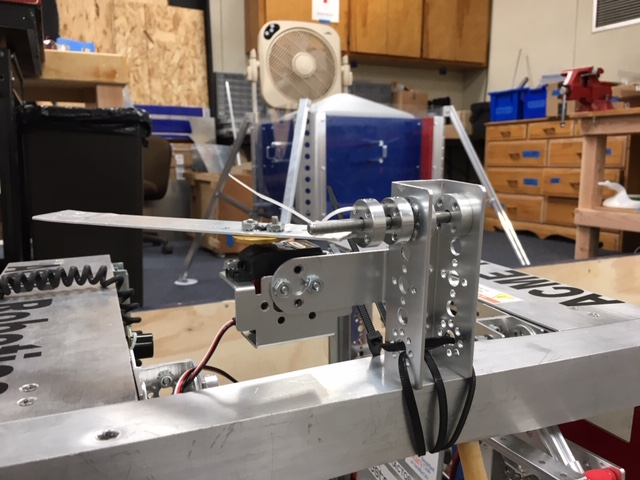
\includegraphics[width=.6 \textwidth]{06_10-08/images/latch1.JPG}
    \caption{Latch Prototype}
    \label{fig: Latch CAD1}
\end{figure}

\begin{figure}
    \centering
    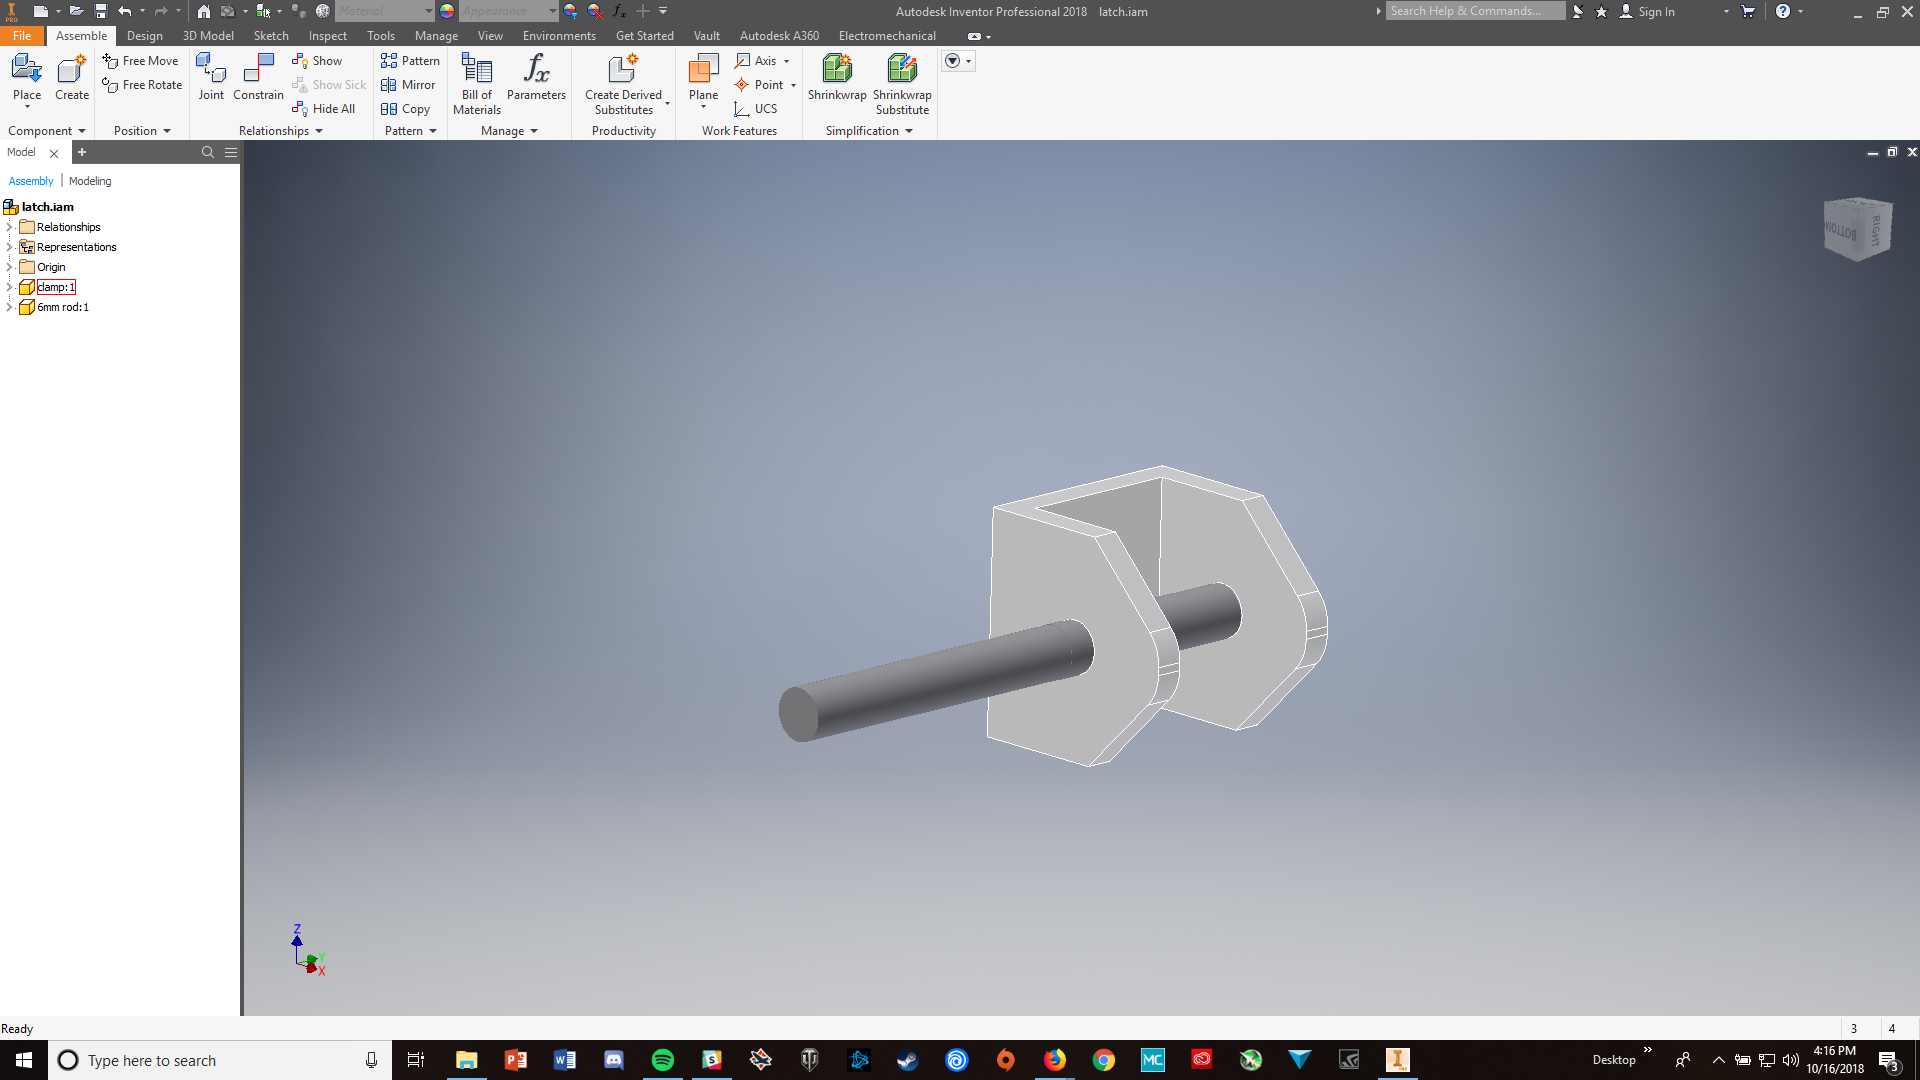
\includegraphics[width=.6 \textwidth]{06_10-08/images/latch.png}
    \caption{Latch CAD}
    \label{fig: Latch CAD2}
\end{figure}

\subsection{H4: Finalize robot design}

The team got together and went over the robot design, making sure that everything had been considered and accounted for before the final stages of CAD were completed and parts were ordered. Everybody presented prototypes and CAD that they had been working on, and the team decided whether or not to stick with it, and discussed any problems that might arise as the parts went into production. The first thing to decide was the type of drive base. The team had used mecanum drives the previous two years, and was confident they could build it correctly, but did not want to dismiss a tank drive. The tank drive that was being considered was a chain driven 6-wheel drop center west coast drive. The mecanum drive being considered was the same thing that the team had used to success last year, a belt-driven mecanum drive, with dead axles constrained between drive plates giving it extra rigidity. Oren had made some improvements over last year's design, including using smaller belts and swapping out parts to increase maintainability. The team decided they should use mecanum drive for its increased maneuverability unless a definite need for tank drive was needed. Because the defensive advantage given by the advantage of tank was countered by the maneuverability of mecanum and the ability to get out of tight situations, and the settled upon intake had no need for the robot to be able to go inside the crater, the team decided to go with a mecanum drive. The team decided to stick with the intake design consisting of a rake that would extend over the crater wall and pull minerals toward the robot and a series of surgical-tubing whips to suck the minerals in from there. The active sorter using a color sensor was chosen because it would be more reliable when the robot was in motion, and the double cartridge design was chosen because it would allow the two mineral types to be scored independently. Finally, the team decided to use the custom lift rather than the x-rail based one because Oren was confident that he would have the time to manufacture it to the neccecary specifications, and Dan felt it was something that would be able to be made on the manual mill at GSS.
\subsection{S1: Continue working on lift kinematics}

This week Emma continued to work on software for the lift. She wrote the code for the other modes that the lift needs to execute. These being the "hold position" and "driver controlled" modes. As stated in her last entry, Emma used a enum to switch between modes. Emma also experimented with motor encoders for the first time. Especially how you can use encoder ticks to find out how far up or down the lift has moved. Below is the code that she wrote. 
\begin{lstlisting}[language=Java] 
    private enum LiftMode{
        DRIVER_CONTROLLED,
        HOLD_POSITION,
        RUN_TO_POSITION;
    }

    private int inchesToTicks(double inches) {
        double ticksPerRev = liftMotor1.getMotorType().getTicksPerRev();
        double circumference = 2 * Math.PI * RADIUS;
        return (int) Math.round(inches * ticksPerRev / circumference);
    }

    private double ticksToInches(int ticks) {
        double ticksPerRev = liftMotor1.getMotorType().getTicksPerRev();
        double revs = ticks / ticksPerRev;
        return 2 * Math.PI * RADIUS * revs;
    }

    private double getLiftHeight(){
        return ticksToInches(getEncoderPosition());
    }

    private void setLiftHeight(double height){
        setEncoderPosition(inchesToTicks(height));
    }
    public void update(){

        double liftPower;
        switch (liftMode){
            case DRIVER_CONTROLLED:
                double start = getStartingPosition();
                double max = getMaxLiftPosition();
                double min = getMinLiftPosition();
                int currentPos = getEncoderPosition();
                setStartingPosition(start);
                setMaxLiftPosition(max);
                setMinLiftPosition(min);
                setEncoderPosition(currentPos);

                if(currentPos > start){
                    liftPower = this.liftPower;

                }else if(currentPos == start){
                    liftPower = this.liftPower;

                } else {
                    liftMode = LiftMode.HOLD_POSITION;
                };
                update();
                break;

            case HOLD_POSITION:
                double liftHeight = getLiftHeight();
                double error = pidController.getError(liftHeight);
                liftPower = pidController.update(error);

                break;

            case RUN_TO_POSITION:
                MotionState currrentState = liftProfile.get(System.currentTimeMillis() - startTime);
                break;
        }
    }
    public void goToPosition(double position){
        liftProfile = MotionProfileGenerator.generateSimpleMotionProfile(
                new MotionState(0, 0, 0, 0),
                new MotionState(position, 0, 0, 0),
                1, 1, 1 //find real values eventually
        );
        liftMode = LiftMode.RUN_TO_POSITION;
        startTime = System.currentTimeMillis();

    }
}
\end{lstlisting}
Of course there is more, as far as the variables and setters and getters, but this should give you the general idea. Through this Emma also realized that relying on getting the motor position to account for where the lift is at all times probably isn't very reliable. So she plans to use a Hall Effect sensor on the lift to narrow the field of possible positions.
\clearpage \newpage \section{Week \thesection} 
\subsection{Business Goals}
\paragraph{B1: Decide what business tasks need to be completed before the Burlingame competition}
 Create tasks in Jira that need to be executed before ACME's first competition.
\paragraph{B2: Finalize the budget with the team captains}
 Decide on the final budget for the build.
\paragraph{B3: Print, sign, address, stamp and send the fundraising letters}
 Completely finish the process of sending out fundraising letters to sponsors.
\paragraph{B4: Start interviewing team members for bios}
 Interview ACME members for their bios in the business notebook.
\subsection{Hardware Goals}
\paragraph{H1: Finish Designing the team marker}
 CAD the team marker.
\paragraph{H2: Complete Sorter and Intake CAD}
 Editing the Sorter and attachments.
\paragraph{H3: Testing Rev Linear Slide Kit}
 Build the linear slide system. 
\newpage
\subsection{B1: Decide what business tasks need to be completed before the Burlingame competition}

With the team's first competition confirmed, Emma thought it might be good to start figuring out what business tasks needed to be completed before hand. Using the business Jira board, Emma wrote up tasks that covered all areas of the business team. Such as, finishing fundraising letters, writing up the goals and action plan in the EN, and writing up ACME's outreach events in the EN. Having a list of tasks written out, whether on paper or on a screen, is better way to keep track of tasks rather than just having a running list in your head. Most of the tasks she created were specific to the EN and need to be completed before their first tournament. She will be working on several of these tasks in the weeks to come.

\subsection{B2: Finalize the budget with the team captains}

Finalizing the budget for the season was important to complete sooner rather than later because so many other tasks (especially business tasks) depended on it. Using the list of parts needed for the robot, the team was able to estimate how much all of the parts would cost (\$2500), including how many extras they were going to need to build spare parts just in case something broke on the robot. The team also left enough room in the budget to allow for iteration, if need be (\$700). That total came out to be \$2,200. As an extra precaution, the team decided to add about 30\% of wiggle room onto that total, bringing the total number to \$6000. The team thinks that this is a very reasonable number and is planning to reach it by sending out fundraising letters to the community. As the team is not supported by any school, it is important to decide the budget as early as possible in order to send them out quickly.

\subsection{B3: Print, sign, address, stamp and send the fundraising letters}

Although the fundraising letters were already written, the team still needed to print them out, address them, and mail them. Emma printed out over 50 individually addressed letters. Then, she, Kelly, and Sean and Eli from ARES signed their names at the bottom of the letters. ACME believes that this looks professional and adds a bit of a personal touch to each letter.  Eli and Sean addressed each envelope and the mentors sent them out later that day, as you can see in figure \ref{fig:Letters}. Both teams are expecting funds to come in the coming weeks. 

\begin{figure}
    \centering
    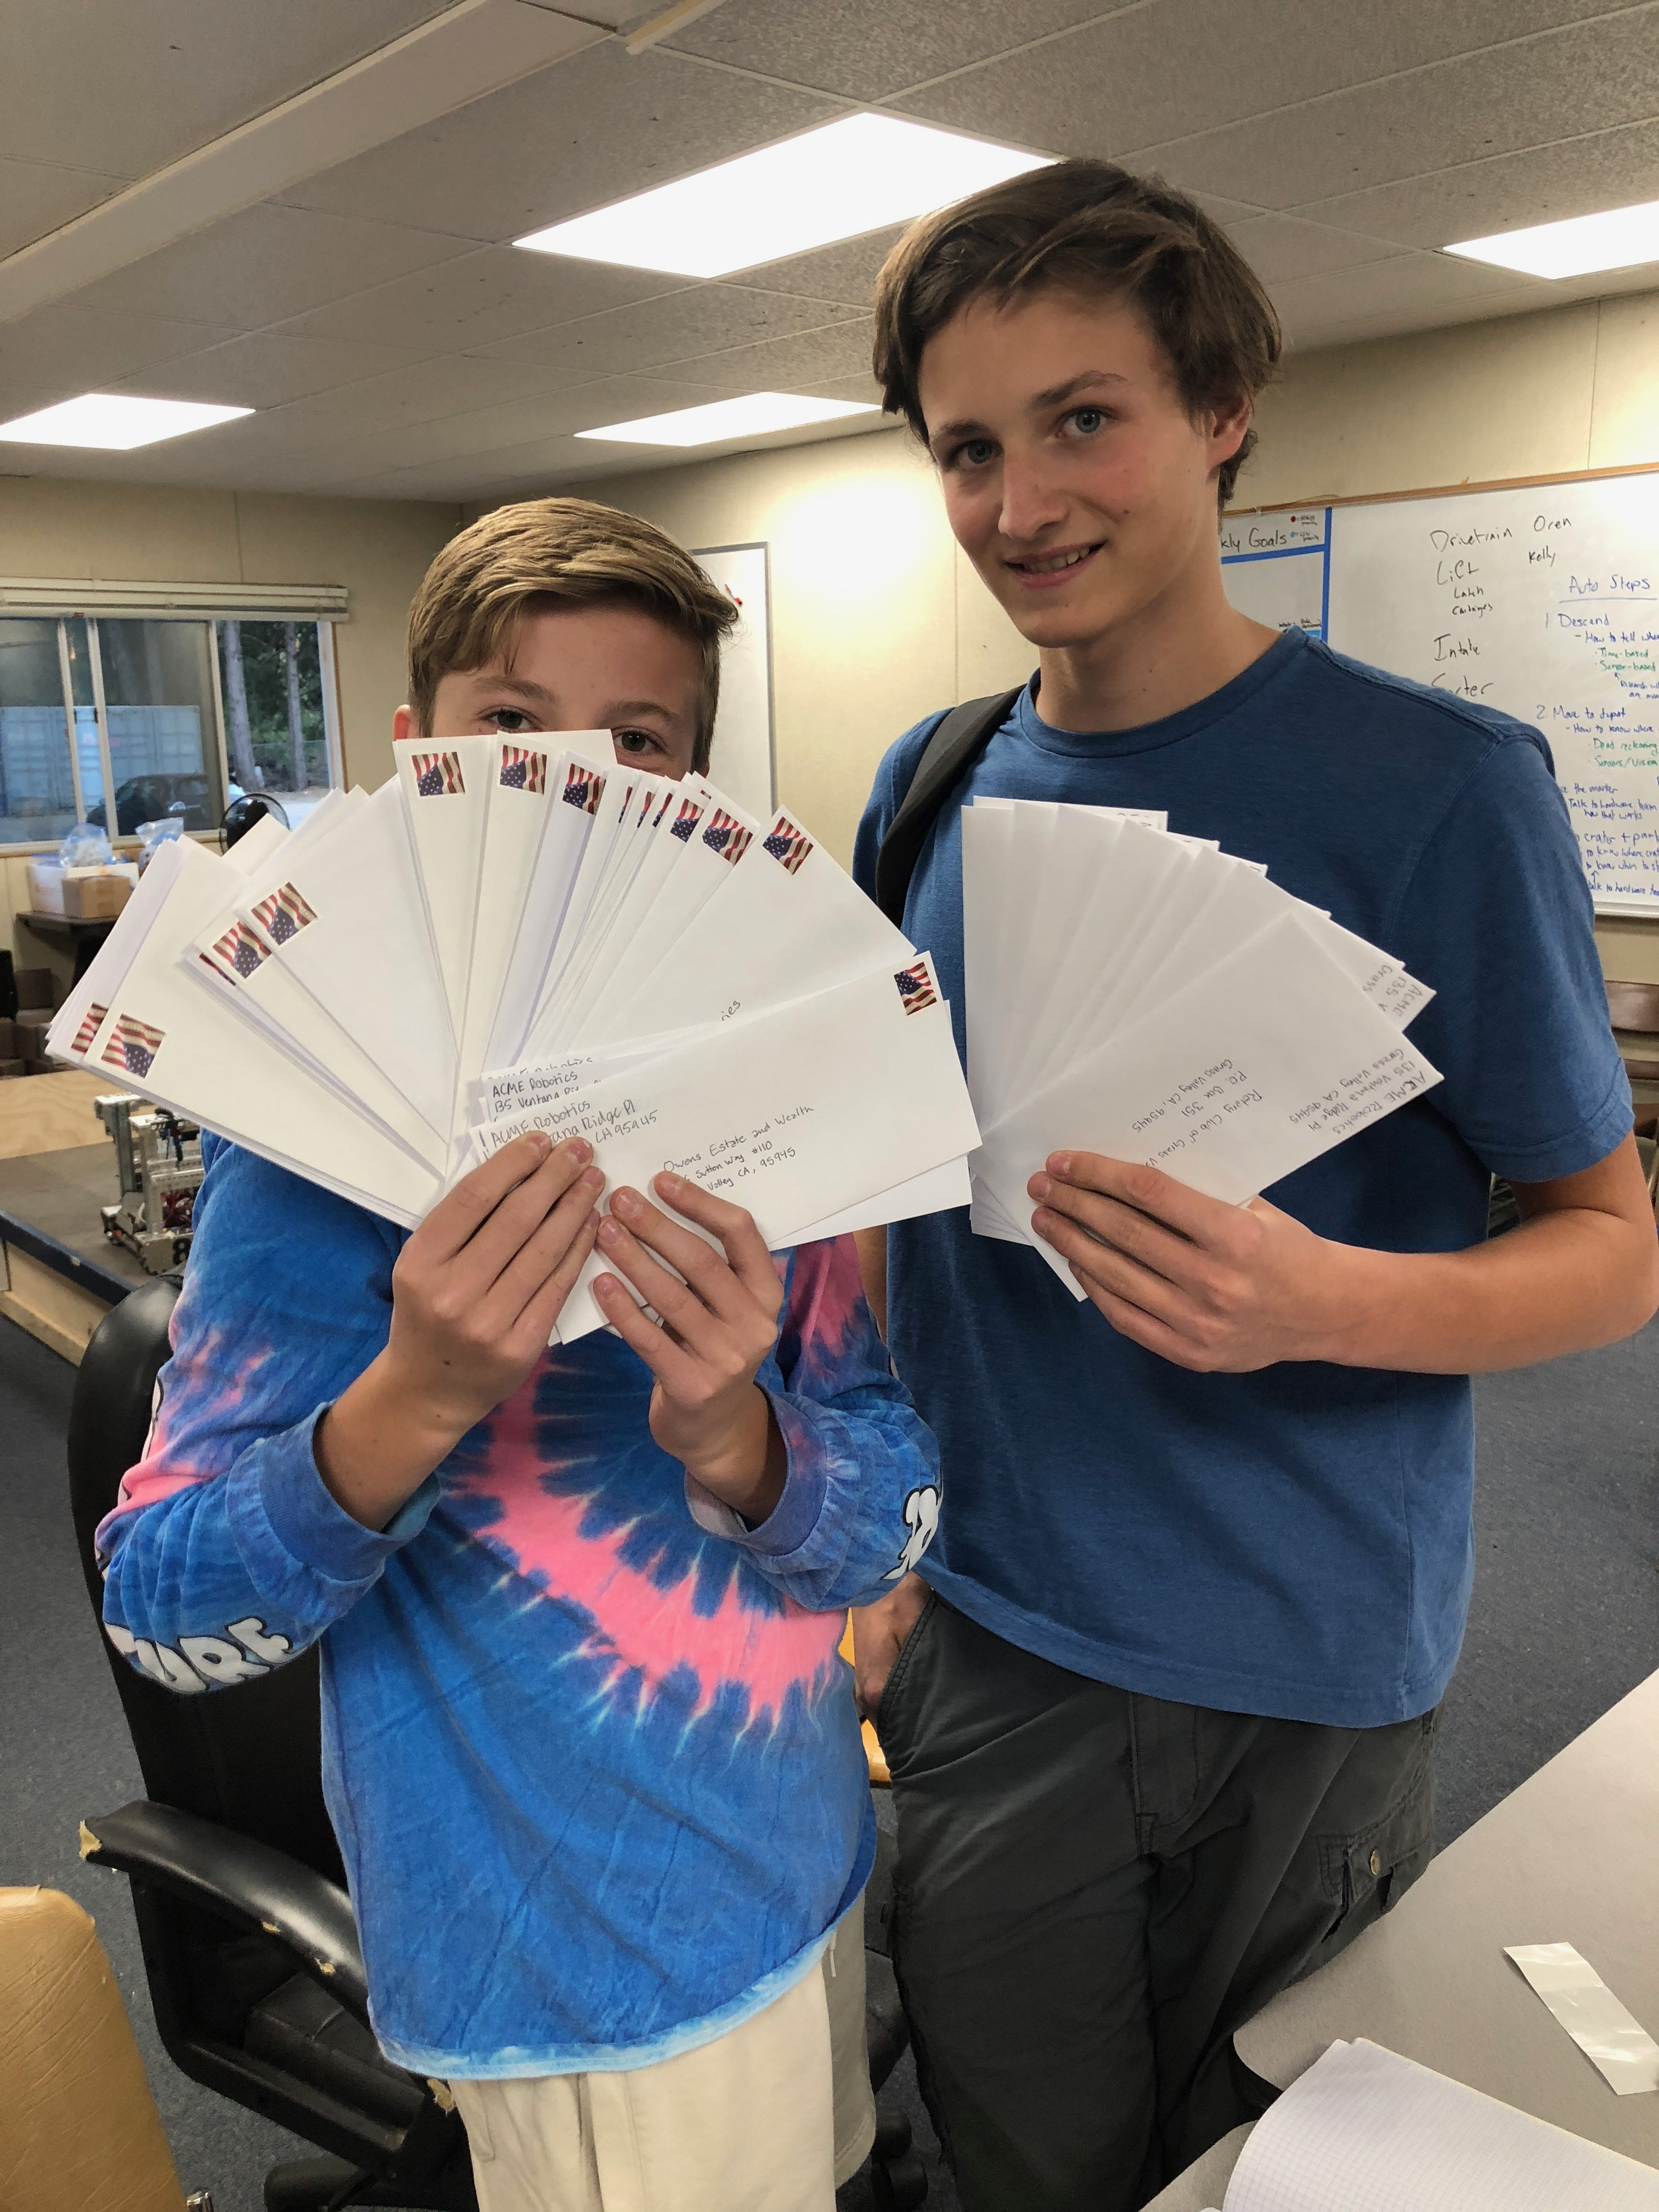
\includegraphics[width=.6 \textwidth]{07_10-15/images/letters.jpg}
    \caption{Eli and Sean with the final letters}
    \label{fig:Letters}
\end{figure}

\subsection{B4: Start interviewing team members for bios}

As always, the most distracting task of the season has come again. This is of course, interviewing members for their bios in the Business Notebook. Why is it so distracting to people? Because listening to Emma and Kelly give an interview to each member is for some reason very entertaining. Besides that they were able to gather all of the information that they needed. Some of the questions asked were, "What is your wildest idea for a FTC challenge?" and "What is your favorite gracious professionalism story?" Emma plans to type these bios up in \LaTeX along with a photo of each team member, as shirts and jackets arrive. 

\subsection{H1: Finish Designing the team marker}

Shawn and Ben worked on developing a new team marker that was an anvil. Ben took the old anvil hat CAD from last year and derived the file and re-scaled it to fit in the proper dimensions. Ben then added a hook and for the mechanism and engraved the top of the anvil with the team marker. They then rendered the model. At the next meeting, they further developed the mechanism.

\subsection{H2: Complete Sorter and Intake CAD}

Ashlin and Aidan worked on finalizing the attachment of the sorter to the intake and the rest of the robot as shown in \ref{fig:Intake CAD}. They put the sorter at a 45 degree angle to so that the objects would naturally go into the sorter and out into the cartridges easily because of the steep angle. Because of this they needed to edit the size of the cartridges so that the cartridges would have enough room to be raised up. They also attached a servo to the bottom of the sorter that it would be what rotates the sorter in either direction depending on if the item is a ball or cube.

\begin{figure}
    \centering
    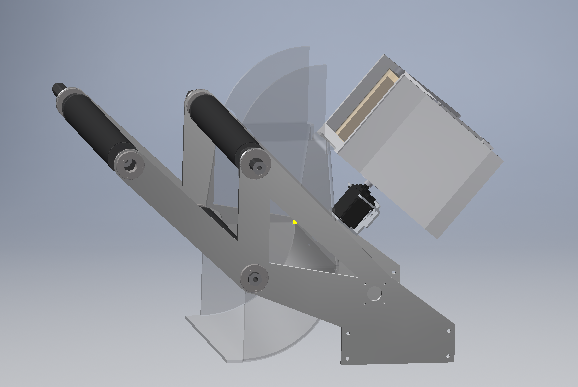
\includegraphics[width=.6 \textwidth]{07_10-15/images/IntakeCAD.png}
    \caption{Sorter and Intake CAD}
    \label{fig:Intake CAD}
\end{figure}

\subsection{H3: Testing Rev Linear Slide Kit}

Recently, the team received the Rev linear motion kits they ordered. To see how exactly the kit went together and see it would be mounted on the robot; Jon put some of the kit together. Jon made several segments, measured, and calculated the exact amount of 15 mm extrusion would be needed for the robot. This gave the team a better idea of how it would be assembled on the robot and a basis for CAD.
\clearpage \newpage \section{Week \thesection} 
\subsection{Business Goals}
\paragraph{B1: Work on the Business Notebook}
 There is much to be done for the BN, so work on it must start immediately.
\subsection{Hardware Goals}
\paragraph{H1: Design of The Deployment Mechanism}
 Making marker deployer.
\paragraph{H2: Turn wheel inserts for the drivetrain}
 Fabricate the wheel inserts.
\newpage
\subsection{B1: Work on the Business Notebook}

The team realized that there was a lot of work that needed to be done on the Business Notebook, so Emma decided to take on that task. The BN includes all of the team's outreach events, the sustainability plan, our goals and action plans, team bios, fundraising information, current sponsor list, etc. With so much to, Emma decided to start with the team bios as those just needed to be typed in \LaTeX . Although there were plenty of answers to questions she and Kelly had asked team members the week before, she only chose 4 or 5 for each bio so that they only filled one page and would leave room for a picture. After the bios were completed, Emma started to write up the outreach events ACME did at the end of last season and over the summer. ACME had been writing about four paragraphs about each outreach event, which Emma thought was a bit excessive. So, she came up with a new format. A picture from the event is at the top of the page followed by the title for the event. A short summary sentence is after that, then bullet points highlighting parts of the event that explain what the team did, how it effected the team and how it benefited the people who the team helped or presented to. She found this method to be much more concise and easy to read. Next week, Emma plans to continue work on the BN by finalizing the budget and writing up the teams goals and action plans. \subsection{H1: Design of The Deployment Mechanism}

Shawn and Ben worked on revising and iterating the marker deployment mechanism. They discussed the best way to easily drop the marker and came up with a bar and hook mechanism.This mechanism works by setting a hook on a bar and then rotating the bar so the hook slides of the end and into the depot.

\subsection{H2: Turn wheel inserts for the drivetrain}

On Monday, Oren and Jon went to Datum Precision Machining to manufacture four wheel inserts which had been previously CADed. The team used Datum because they had a lathe that they were willing to let ACME use. Oren and Jon were not familiar with using a lathe so the owner of Datum, Jon, showed them the basics of operating a lathe. This was important because not only did critical parts for the robot made, but ACME created better ties with Datum and picked up useful skills. Now the team can hopefully continue to work with Datum when it needs parts manufactured. Oren and Jon knowing the basics of turning adds another tool in ACME’s belt as well as bolstering Oren’s and Jon’s individual know how.

\begin{figure}
    \centering
    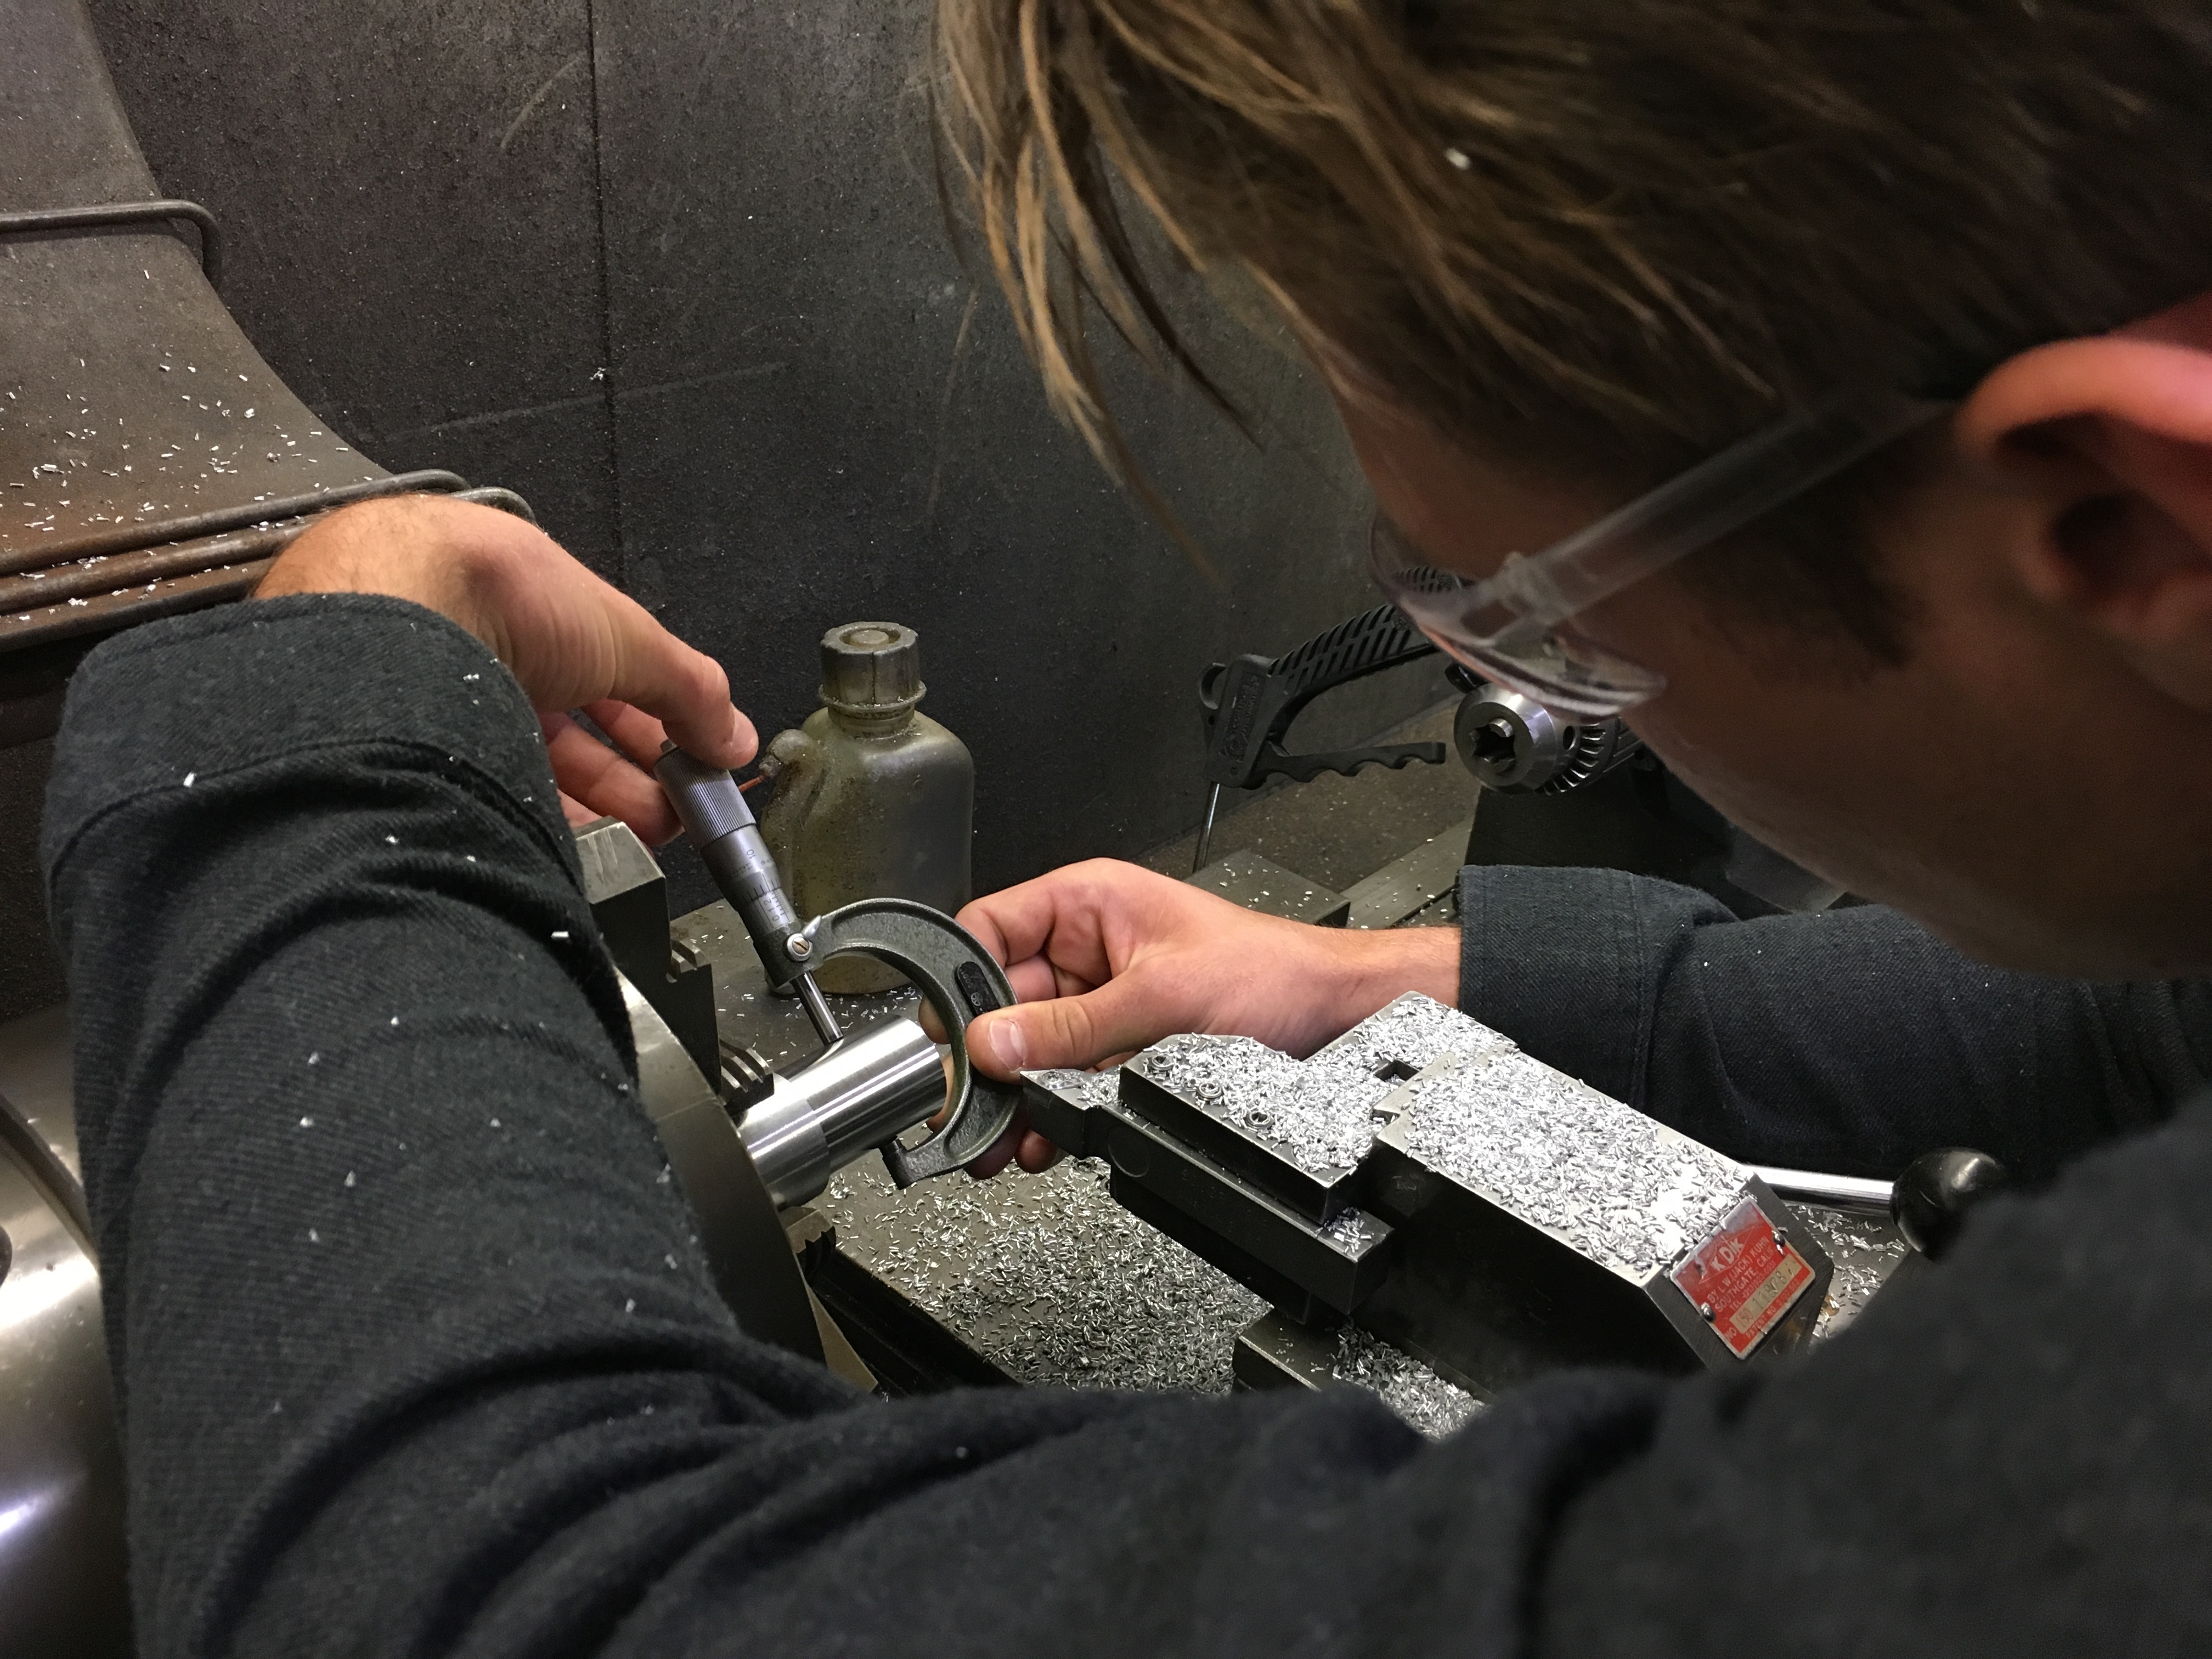
\includegraphics[width=.6 \textwidth]{08_10-22/images/IMG_0330.JPG}
    \caption{Oren checking part measurements}
    \label{fig: Turning Inserts}
\end{figure}

\clearpage \newpage \section{Week \thesection} 
\subsection{Business Goals}
\paragraph{B1: Continue work on the Business Notebook}
 Finish the budget, goals and action plan, and the finishing touches on outreach events.
\subsection{Hardware Goals}
\paragraph{H1: Print the Marker}
 Give Kelly the marker CAD to be printed
\paragraph{H2: Fabrication}
 Start to fabricate the parts for the robot.
\paragraph{H3: Lift }
subsection{Lift 
\newpage
\subsection{B1: Continue work on the Business Notebook}

It was very important to the team to print the Business Notebook at least 24 hours before the team left for the tournament. This meant that in order to meet that goal most of the big stuff that needed to be put into the Business Notebook (budget, goals and action plan, etc.) needed to be done quickly. Emma worked on writing up these things in the BN this week. First, she finalized the budget with the other team captains and mentors and added a few additional expenses such as the cost of the field. Then she put all of this information into a table that could be easily read and understood. For the goals and action plan Emma worked with Stephanie to come up with a new way to display the team's plans for the future. Basically, each goal is listed and given a short summary, then the plans to meet that goal are written in bullet form and then several paragraphs below that illustrate how the team is working to complete the goal or the results of that plan. Emma also added a section to the outreach events about future events that the team is planning. Such events include a presentation to the local Girls Who Code club, a meet up with a VEX robotics team in the county and a workshop with the Girl Scouts. (For more information on these events and other outreach events, please peruse the Business Notebook). \subsection{H1: Print the Marker}

This week Ben finished revising the model of the team marker in Inventor Pro 2018. He then converted the .iam file to an .stl file to be printed. Then, he gave Kelly the file to be printed. Towards the end of the meeting, Ben tapped about 10 churros to be used in the drive train. Figure \ref{fig:marker} shows the final marker. 

\begin{figure}
    \centering
    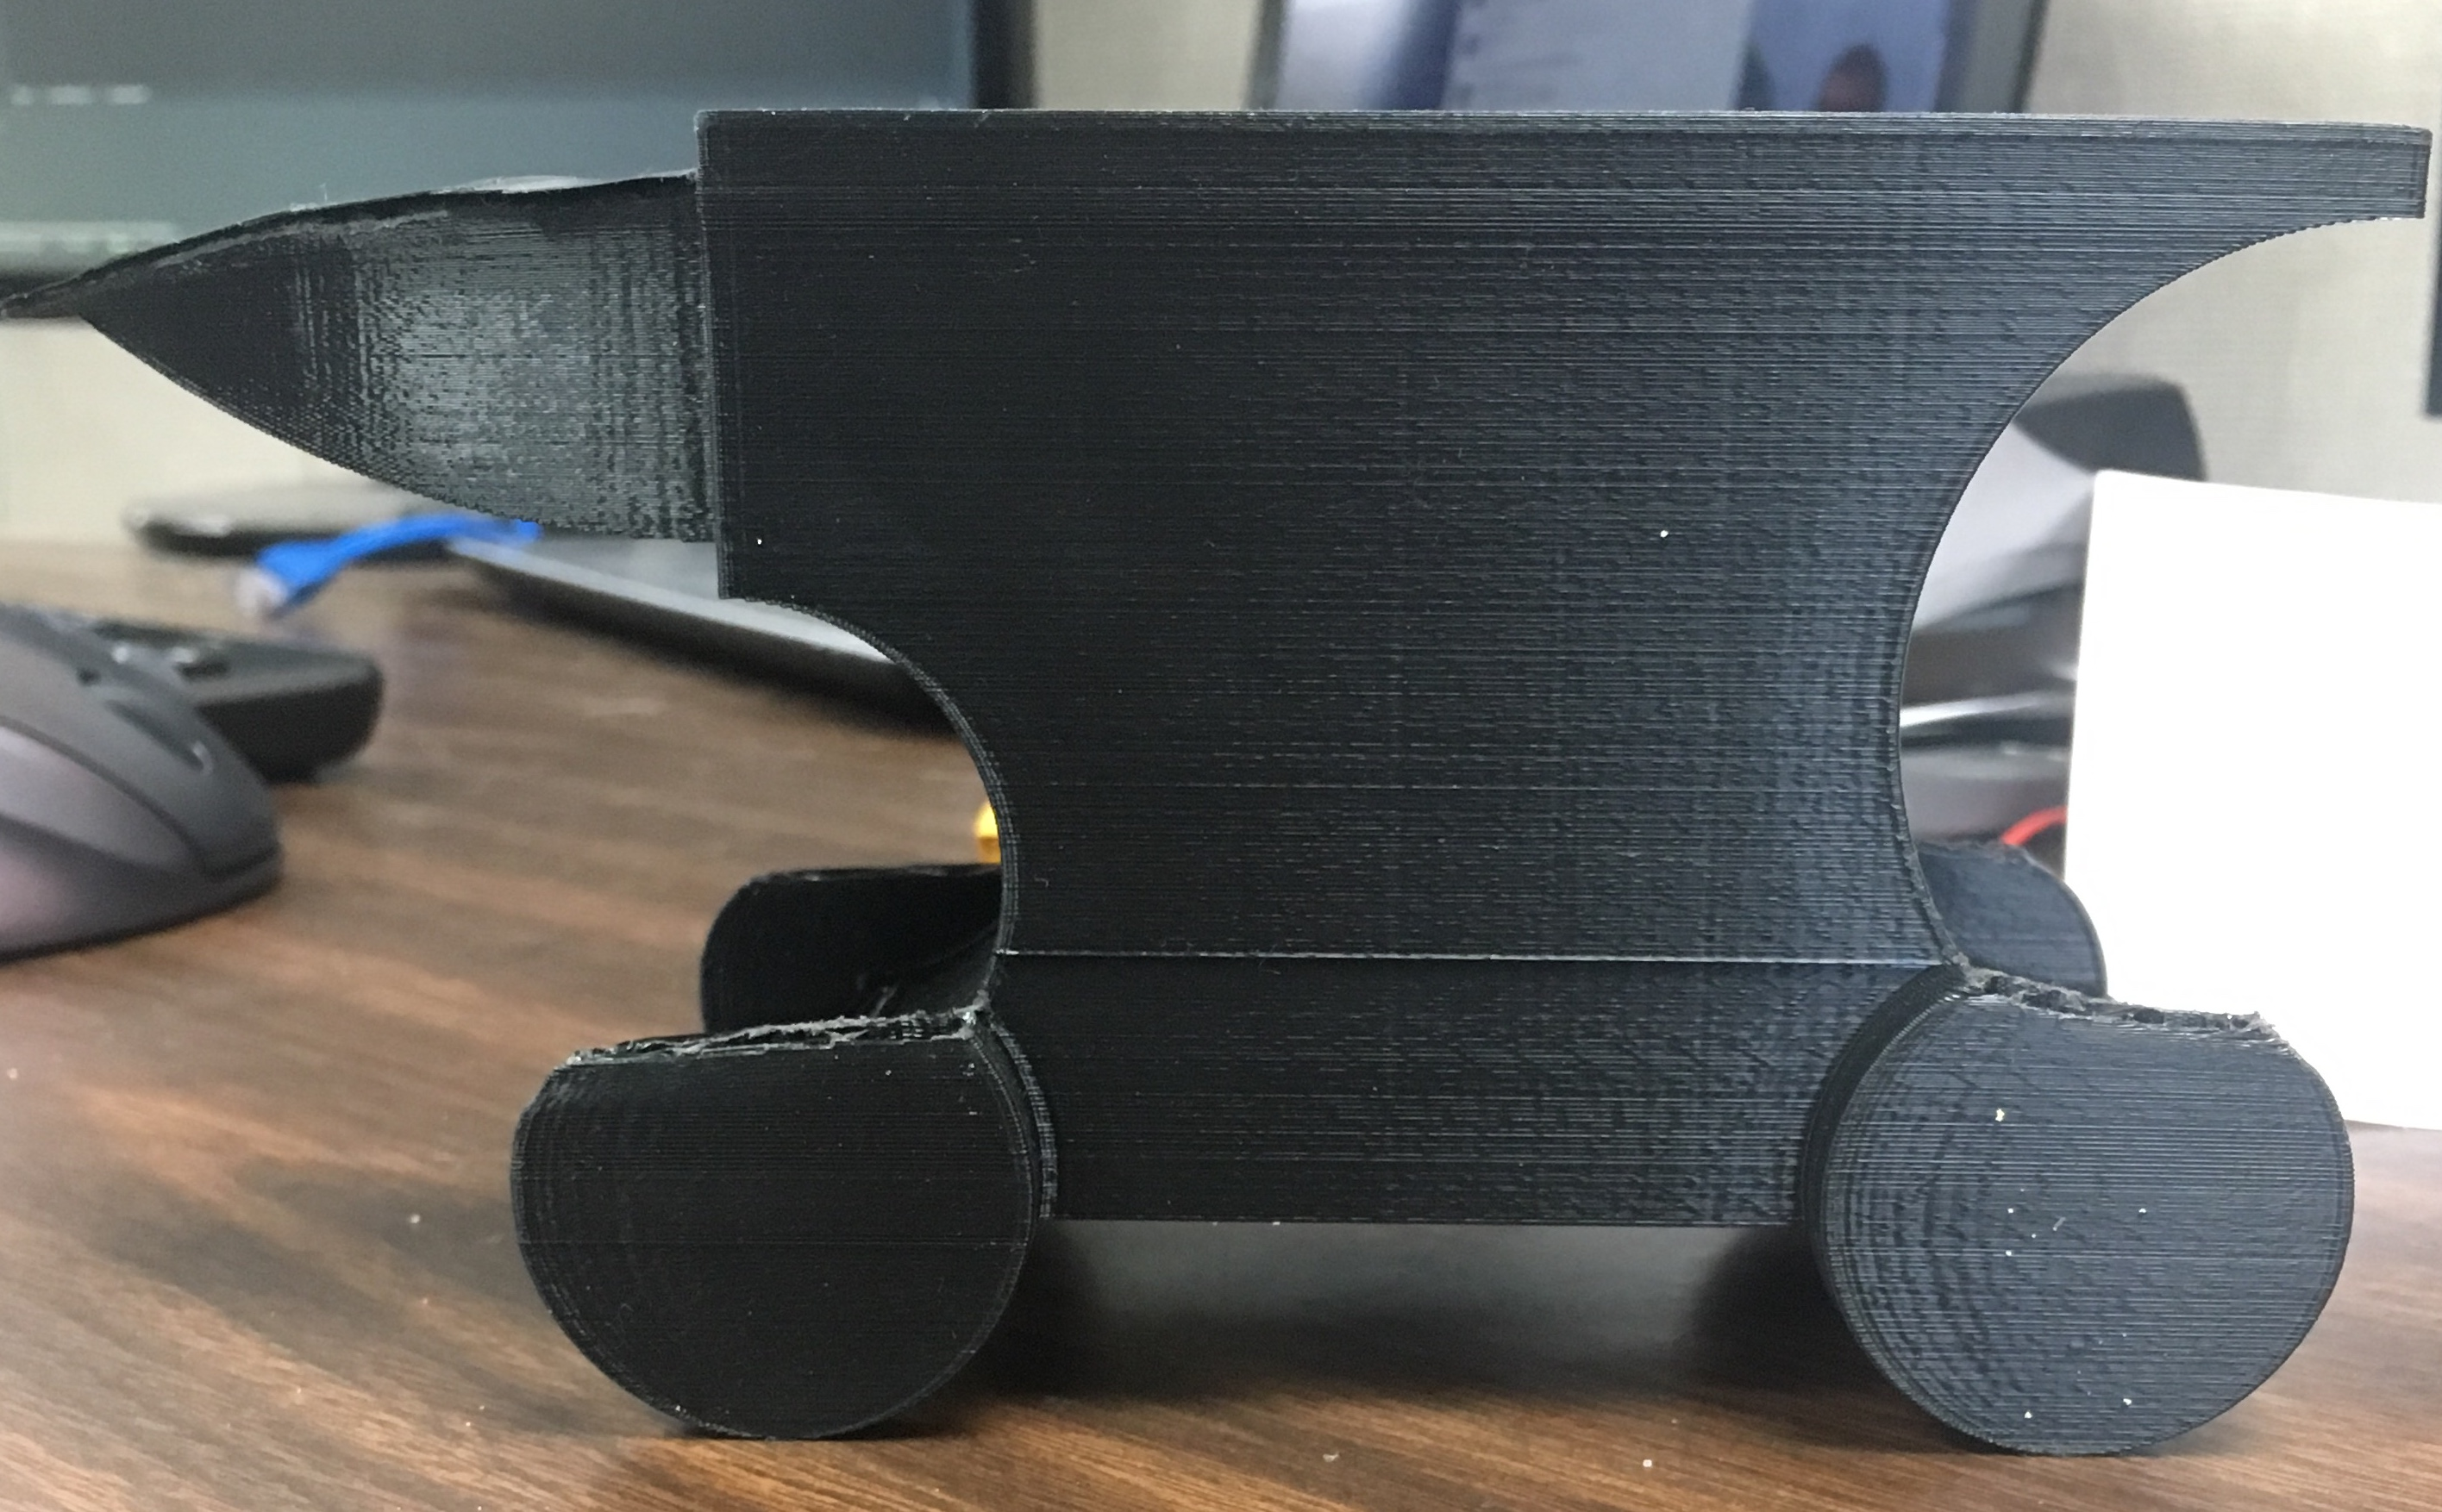
\includegraphics[width=.6 \textwidth]{09_10-29/images/anvil_marker.jpg}
    \caption{Anvil Marker}
    \label{fig:marker}
\end{figure}

\subsection{H2: Fabrication}

Now that the team had most of the parts of the robot, they could begin fabricating the robot. To assemble the intake and drivetrain, the metal cross beams and Vex rollers needed to be cut down to size. Jon had a chop saw and band saw at his house so he took the Vex rollers and cross beams home to be cut. To complete the rollers for the intake, holes had to be drilled in the rollers for the surgical tubing. After drilling a test piece, Jon had to rearrange the way the rollers were clamped in the vice. He then drilled the rest of the Vex rollers.
\subsection{H3: Lift }
}\clearpage \newpage \section{Week \thesection} 
\subsection{Business Goals}
\paragraph{B1: Add finishing touches to the Business Notebook}
 Finish the Appendices and do a final read through of the Business Notebook.
\paragraph{B2: ACME Board}
 Finish the pit board that the team is going to take to the Burlingame tournament.
\subsection{Hardware Goals}
\paragraph{H1: Lift manufacturing}

\paragraph{H2: Sorter Finalization}
 Complete last edits to the sorter.
\paragraph{H3: Intake shield}
 Manufacture and make intake shield.
\paragraph{H4: Drivetrain Assembly}
 Assemble the drivetrain.
\newpage
\subsection{B1: Add finishing touches to the Business Notebook}

The final part of the Business Notebook was writing the Appendices. The Appendices are very important because they include all of the extra information that doesn't fit other sections in the notebook. For example the fundraising letters are put in to the appendix because they are very long and don't fit perfectly in the section where fundraising and sending the letters is mentioned. Therefore, they are referenced in those places but the real letters are at the back of the notebook. This is the same story for the budget details. There is a general budget in the budget section but the individual purchases are in the appendix. \\
The final thing to do with the BN is to read through it once more, fix typos, add a few more photos and print the notebook. Emma took team and mentor photos for the bios and then a team photo for the "team" section. After that was done, she downloaded the BN PDF and printed the notebook. There are still a few things to add in order for the notebook to be completely done, such as write the summary page and space out the sections with dividers, but the goal to print the notebook at least a day before the tournament was met!

\subsection{B2: ACME Board}

This week, Ben was tasked with making the ACME board. To do this he typed up multiple short paragraphs about subsystems, outreach, and software. Then he printed them out along with photos that show a visual. In Figure \ref{fig:pitboard} you can see the sketch that Ben made of the layout of the board. 

\begin{figure}
    \centering
    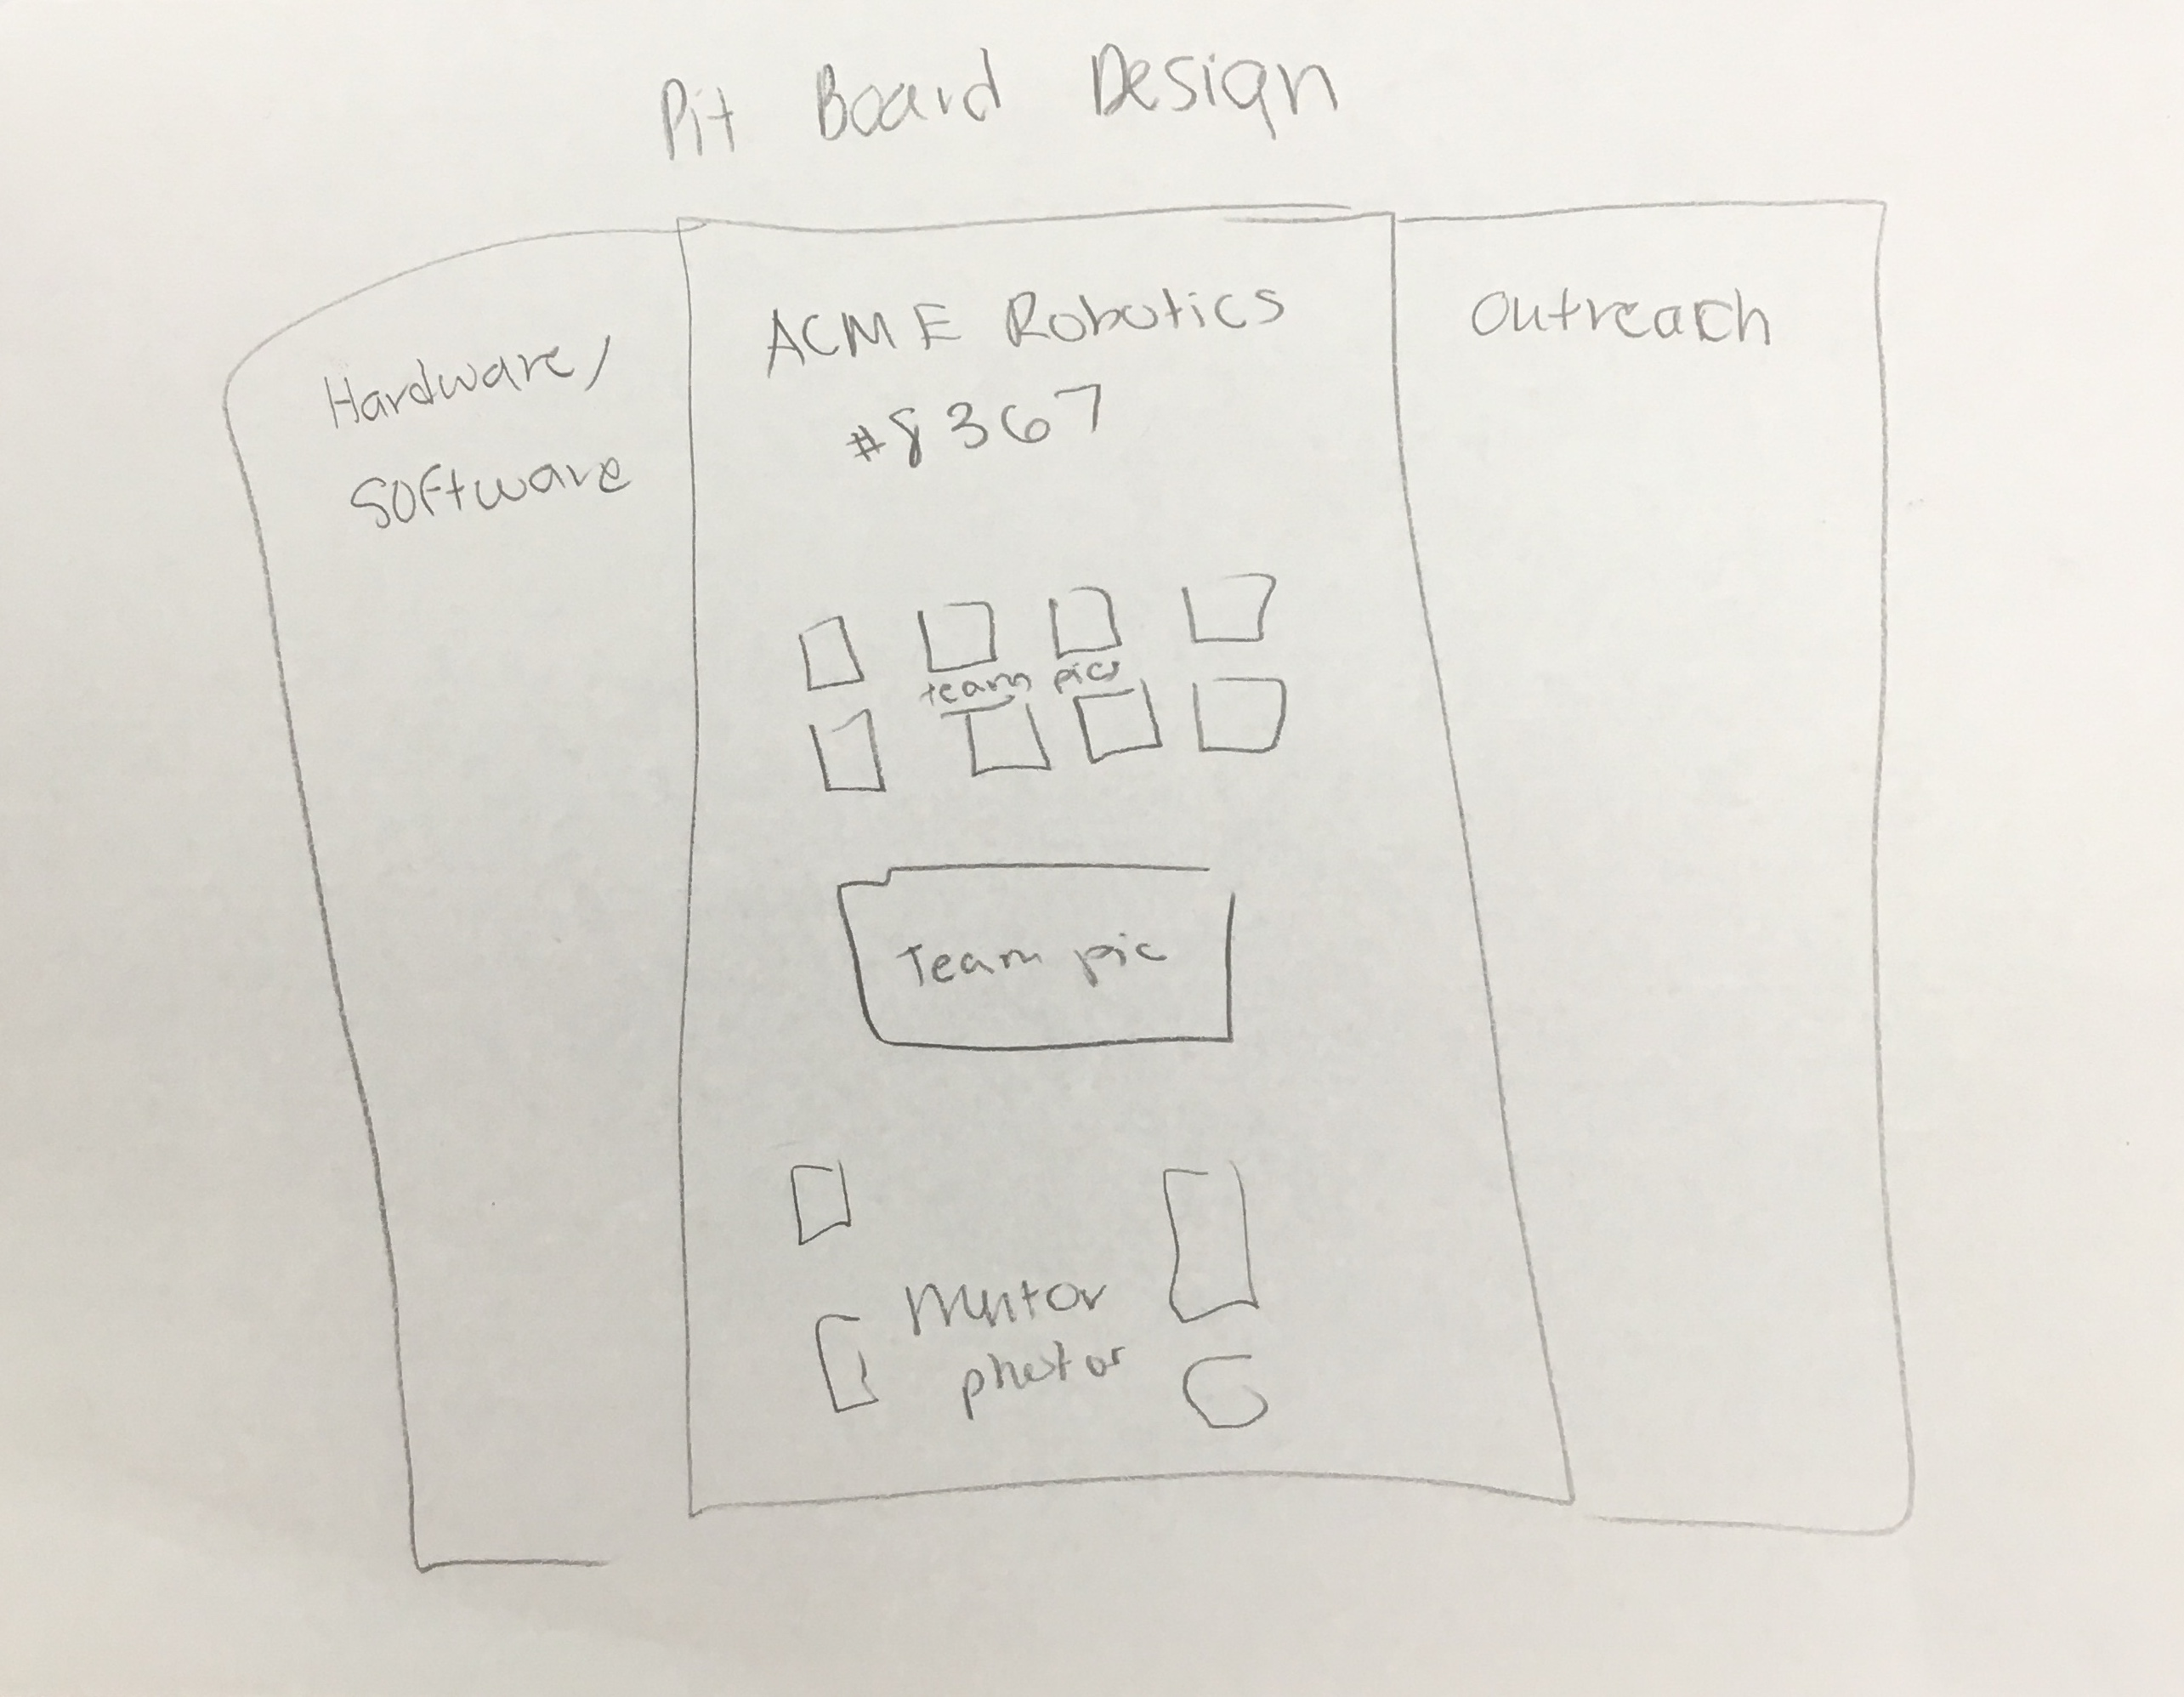
\includegraphics[width=.6 \textwidth]{10_11-05/images/pit_board.jpg}
    \caption{Pit Board Sketch}
    \label{fig:pitboard}
\end{figure}
\subsection{H1: Lift manufacturing}

 After the finalization
 
\subsection{H2: Sorter Finalization}

The sorter needed to be printed as soon as possible so Ashlin and Aidan made some finalizing touches to the sorter so that it could print. First they split it the base design into two parts making the top be its own piece. They did this so that the top could be removed to allow for the swiveler to be put in the sorter and also so that the top piece could be printed separately to allow for the print to be easier. They also edited the top piece so that a bearing could fit into it tightly which would allow for the overall rotation of the sorter to be that much smoother. They printed the sorter on one of their sponsor's printers (see Figure \ref{}).

\begin{figure}
    \centering
    \includegraphics[width=.6 \textwidth, angle=270]{10_11-05/images/sorter.JPG}
    \caption{Sorter and Intake CAD}
    \label{fig:Intake CAD}
\end{figure}

\subsection{H3: Intake shield}

After the intake shield was cut Ashlin and Aidan heat bent the shield so that it would be shaped exactly as the 3D model. After the shield was bent they tested it to make sure it successfully in-took balls and cubes. The testing was successful and the shield worked  spectacularly.

\begin{figure}
    \centering
    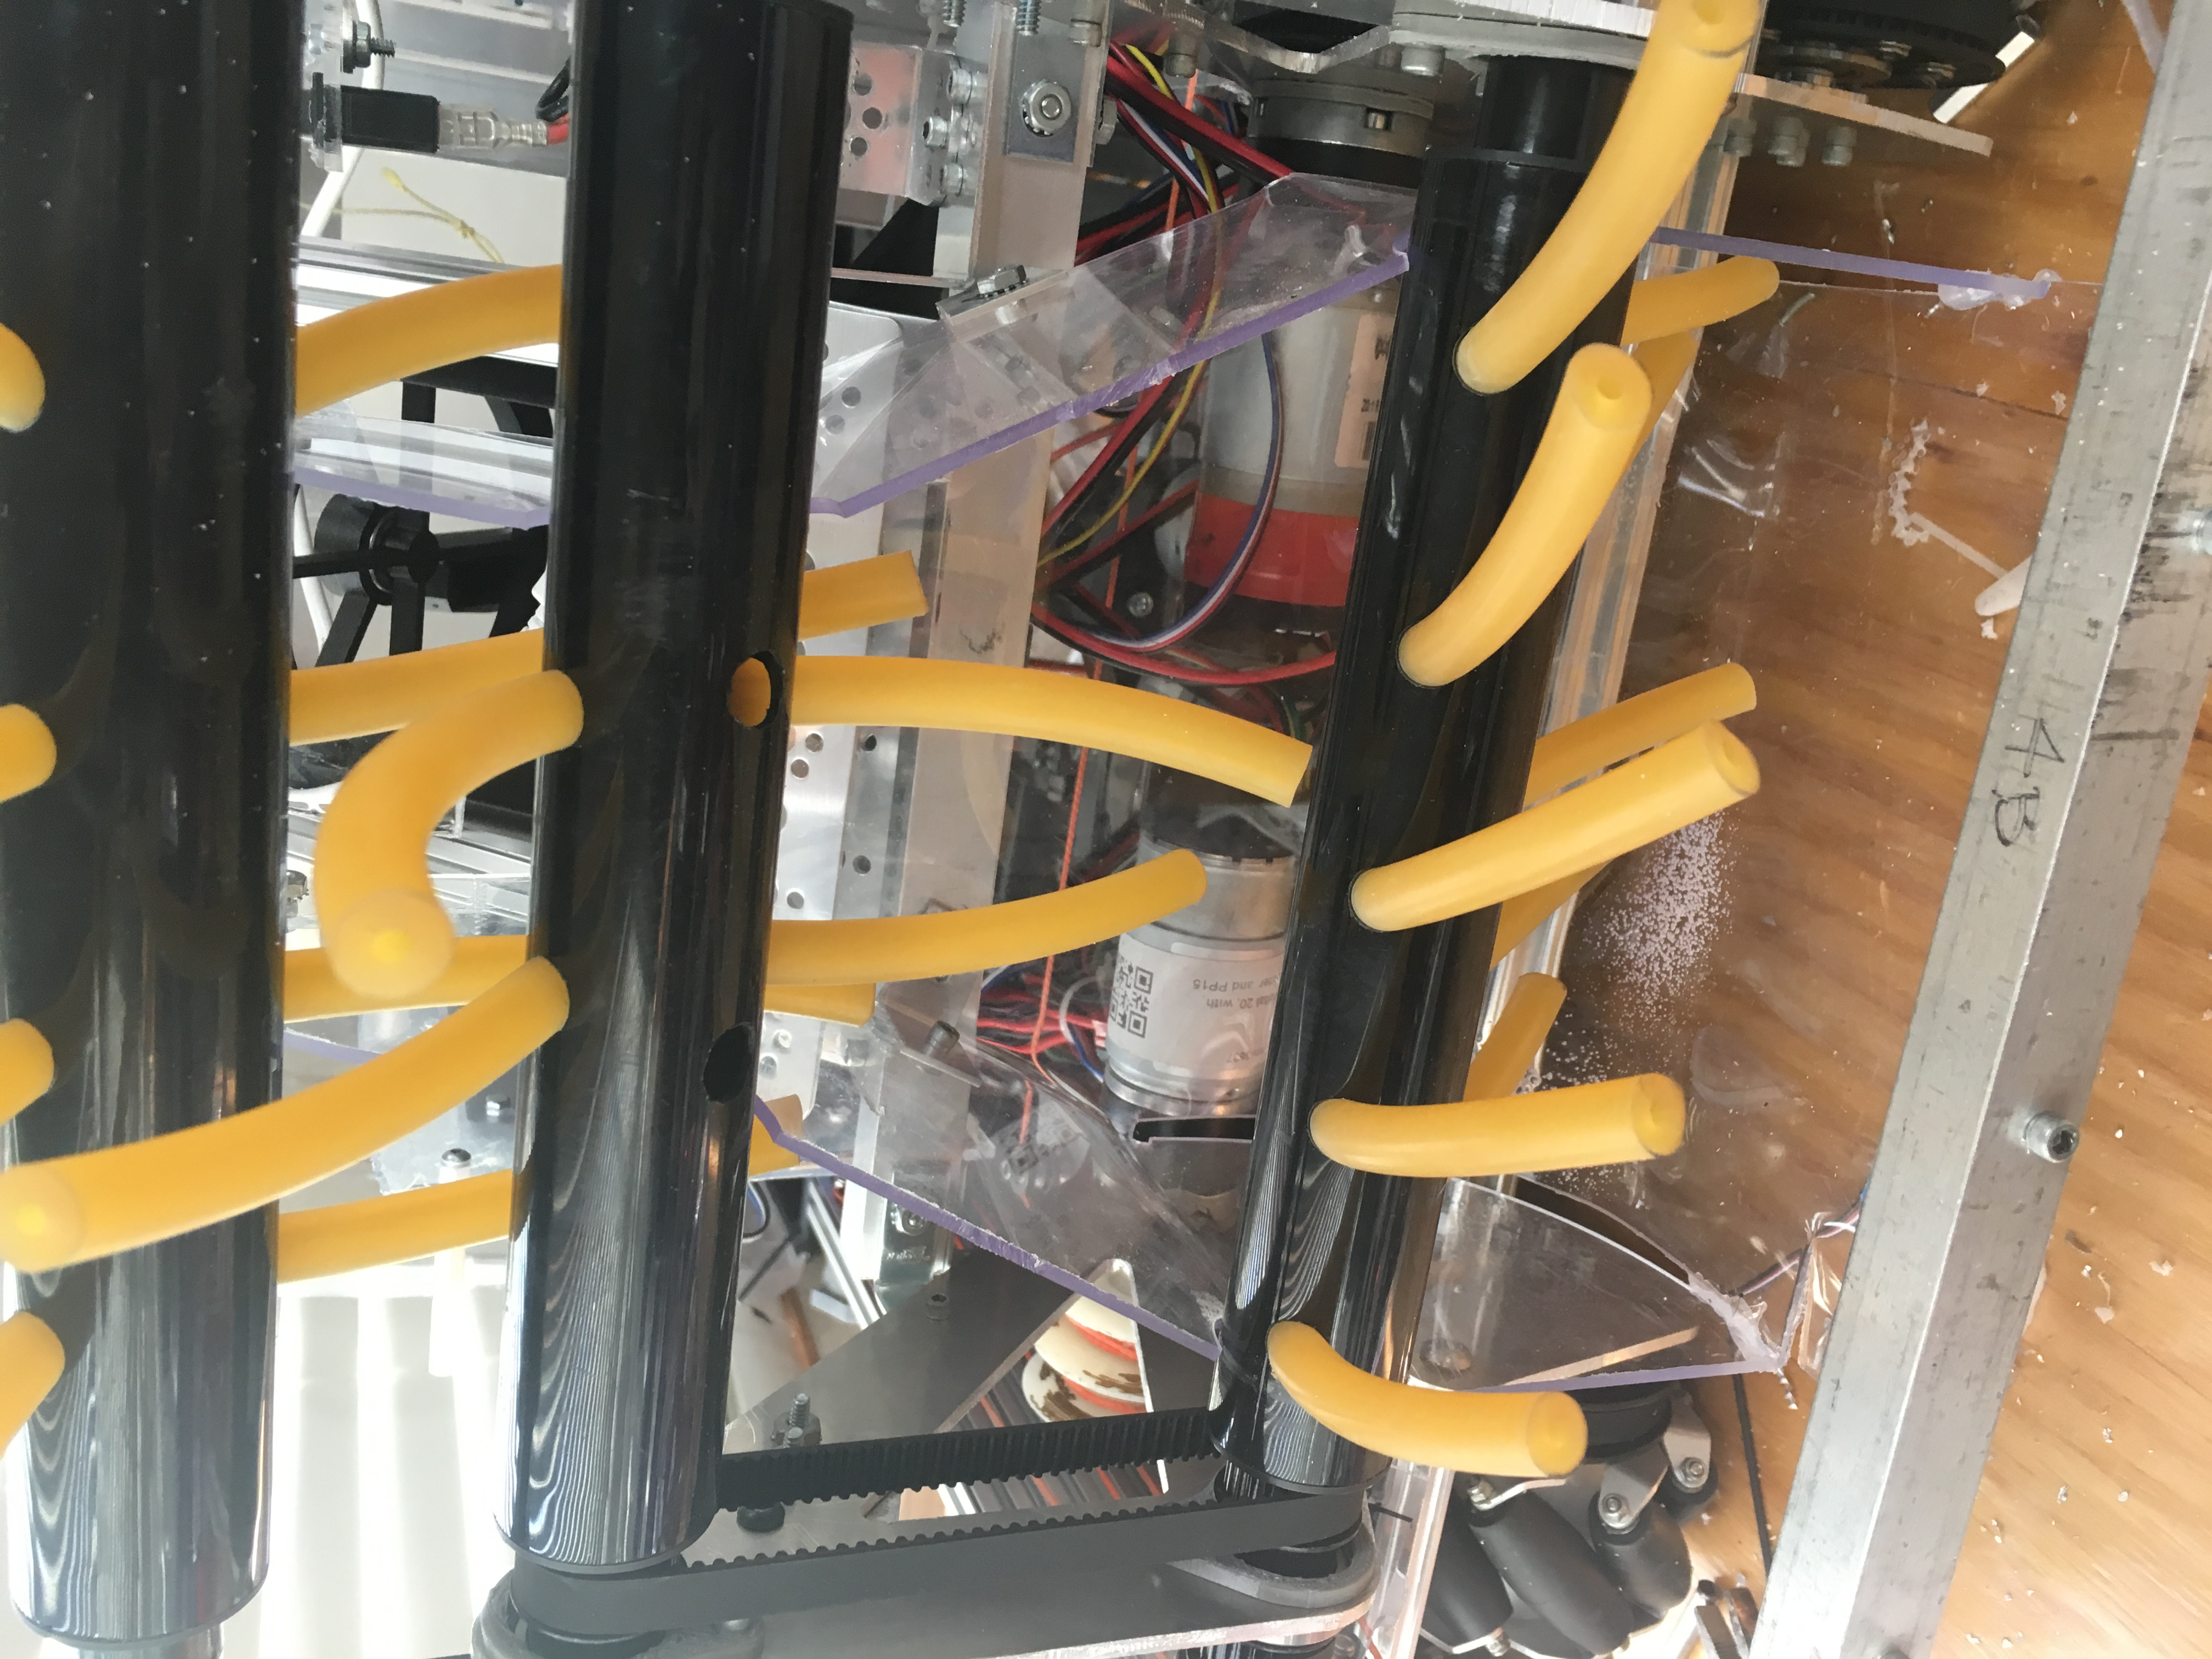
\includegraphics[width=.6\textwidth, angle=270]{10_11-05/images/intake_shield.JPG}
    \caption{Intake Shield}
    \label{fig:Intake Shield}
\end{figure}

\subsection{H4: Drivetrain Assembly}

This week Oren manufactured the drivetrain. He used a mill to cut out all of the plates. He ran into some hard parts along the way that includes custom motor mounts, making sure everything was as accurate as possible, and lock tight every screw.

\begin{figure}
    \centering
    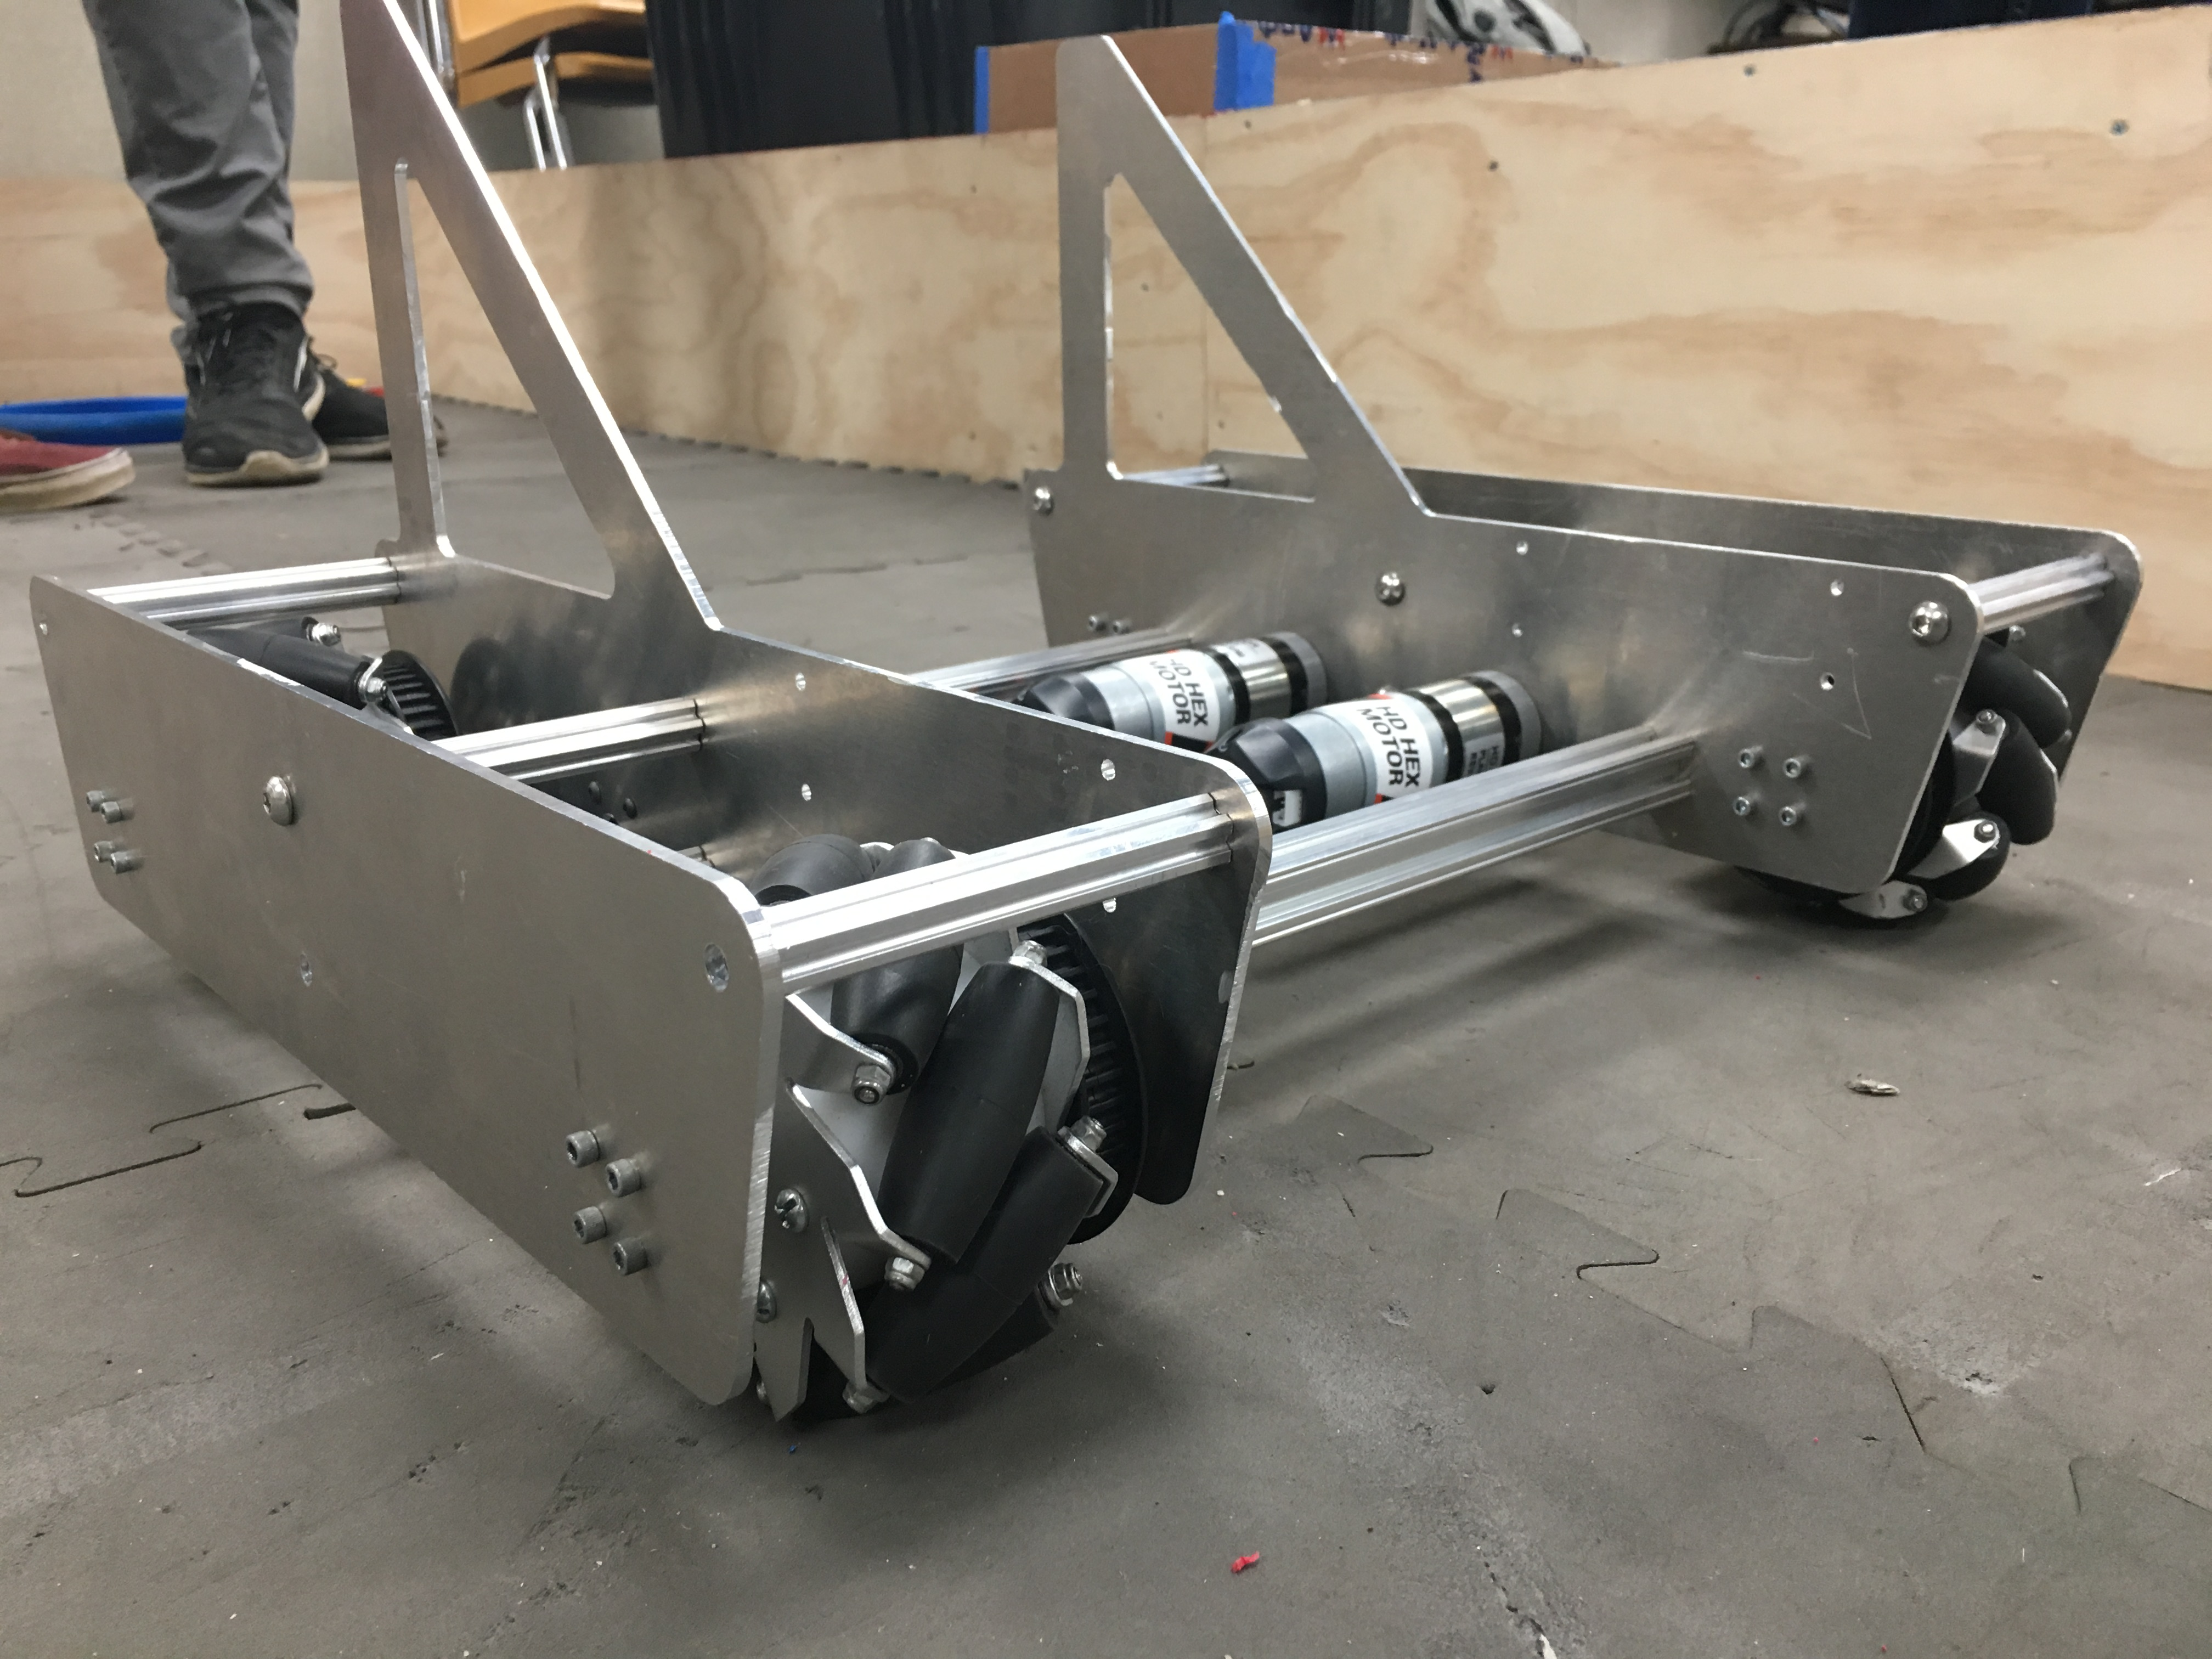
\includegraphics[width=.6 \textwidth]{10_11-05/images/drivetrain.JPG}
    \caption{Drivetrain}
    \label{fig:drivetrain}
\end{figure}
\clearpage \newpage \section{Week \thesection} 
\subsection{Business Goals}
\paragraph{B1: Write the summary and cover pages for the Business and Engineering Notebooks}
 Finish up the BN by printing the summary and cover pages.
\subsection{Hardware Goals}
\paragraph{H1: Assembling Rev Linear Motion Slides for the Rake}
 Assembling and Attaching the Linear slides and Rake system.
\paragraph{H2: Shield Attachment}
Attaching the Shield to the robot.
\newpage
\subsection{B1: Write the summary and cover pages for the Business and Engineering Notebooks}

As the tournament draws closer, finishing the Business Notebook becomes ever more important. Even though the notebook itself was already printed, a cover page and summary page was still needed to complete the task. Emma worked on the summary page this year. The summary page is not only an introduction to the team's mission, it is where specific parts of the notebook worth noting can be found, as well as specific events. Emma adapted the summary page the team used last year by rewriting the team's story and mission for this year, altering the season highlights, and choosing specific topics of interest in the notebook. The season highlights are notable events that are exciting or great accomplishments of the team. The team's overlying goal for this year is to maintain the FIRST program in our community and train members on our team so that ACME can keep going in the future. The summary also mentioned goals on how the team wants to progress to Worlds again this year. With these things complete, the BN is now complete.  


\subsection{H1: Assembling Rev Linear Motion Slides for the Rake}

Continuing the manufacturing process, Jon and Aidan assembled the linear slides for the intake rake. The team wanted to create a four stage slide so that no matter where the robot was around the crater it could reach every cube or ball in the crater. However the team had only bought two linear slide kits which would only allow for a two stage slide. John and Aidan found extra parts from the previous years linear slide system. This allowed for there to be a three stage system which would give them enough length to reach to almost the back of the crater and get plenty of minerals. After constructing the slides, Jon and Aidan had to fine tune them to get them both to run smoothly and with little resistance because there was only going to be one motor powering both slides and if there was too much resistance the motor wouldn't be able to power them. After these were constructed, Aidan went on to build the rake portion of the slide and Jon attached the slides to the robot. Jon did this by using Tetrix L brackets and screwing them into the outside plate of the drive train. This made sure the slides were inside the 18 inches and were firmly attached to the robot in case they got bumped by another robot during competition. To create the rake Aidan needed to find a way to minimize the length it added to the robot. The rake had to sit low enough so that it could tuck under the intake system but it needed to be high enough so that it would pass over the crater wall. Aidan solved this by having the axle of the rake sit exactly 4 inches above the ground.

\subsection{H2: Shield Attachment}

After the shield was built it needed to be attached to the robot. The attachment piece would attach to the side plates of the intake But couldn't attach to the back of the sorter because the screws on the attachment might catch cubes when the went up the intake. To solve this Aidan created brackets that would allow the attachment piece to screw into the shield on the sides which would decrease the likely-hood of cubes getting caught.\end{document}